\documentclass[11pt]{article}

% ============================================================================
%  Rub' al-Khali soil metagenome -- MANUSCRIPT v2, rewritten 2026-09-17.
%  v1 is archived at main_v1.tex and no prose is carried over from it.
%  Historical claims: notes/CATALOGUE_NUMBERS.md and notes/CORRECTIONS.md.
%  October review revisions: reproducibility/darkmatter/current_claims.tsv,
%  retained input manifests and reviews/darkmatter-2026-10-13/.
%  Whole-paper registry migration and public data release remain incomplete.
% ============================================================================

\usepackage[a4paper,margin=2.4cm]{geometry}
\usepackage{graphicx}
\usepackage{booktabs}
\usepackage{array}
\usepackage{authblk}
\renewcommand{\Authfont}{\normalsize}
\renewcommand{\Affilfont}{\small}
\usepackage{xcolor}
\usepackage[numbers,sort&compress]{natbib}
\usepackage{hyperref}
\hypersetup{colorlinks=true,linkcolor=blue!50!black,citecolor=teal!60!black,urlcolor=blue!50!black}
\setlength{\emergencystretch}{2em}

\providecommand{\todo}[1]{\textcolor{red}{\textbf{[TODO: #1]}}}
\newcommand{\unreg}[1]{\textcolor{orange!80!black}{#1}}   % computed, not yet registered

\title{\textbf{Widespread desert archaea harbour a disproportionate share of unknown protein families}}
% Same authors and affiliations as Life on Air; order specified by Robert, 15 October 2026.
% Alejandra first; middle authors alphabetical by surname; Magnus and Robert last.
\author[1]{Alejandra Lopez Velazquez}
\author[1]{Marwa Abdelhakim}
\author[3]{Sulaiman M. Alajel}
\author[1]{Mohammed Alarawi}
\author[1]{Hind Aldakhil}
\author[1]{Abderahmane Derouiche}
\author[5]{Daniela I. Drautz-Moses}
\author[4]{Michel Dumontier}
\author[7]{Raik Grünberg}
\author[1]{Maxat Kulmanov}
\author[2]{Susana Martinez Arbas}
\author[1]{Kexin Niu}
\author[1]{Krishnakumar Sivakumar}
\author[1]{Rund Tawfiq}
\author[6]{Tiannyu Wang}
\author[5]{Xiang Zhao}
\author[1]{Jood Kamal Zubair}
\author[6]{Magnus Rueping}
\author[1]{Robert Hoehndorf\thanks{Correspondence: robert.hoehndorf@kaust.edu.sa}}

\affil[1]{Bio-Ontology Research Group (BORG), Computer, Electrical and
  Mathematical Sciences and Engineering (CEMSE) Division, King Abdullah
  University of Science and Technology (KAUST), Thuwal, Saudi Arabia}
\affil[2]{Luxembourg Centre for Systems Biomedicine (LCSB), University of
  Luxembourg, Esch-sur-Alzette, Luxembourg}
\affil[3]{Ministry of Environment, Water and Agriculture, Saudi Arabia}
\affil[4]{Institute of Data Science, Department of Advanced Computing
  Sciences, Faculty of Science and Engineering, Maastricht University,
  Maastricht, The Netherlands}
\affil[5]{Bioscience Core Lab, King Abdullah University of Science and
  Technology, Thuwal, Saudi Arabia}
\affil[6]{Physical Science and Engineering (PSE) Division, King Abdullah
  University of Science and Technology (KAUST), Thuwal, Saudi Arabia}
\affil[7]{Biological and Environmental Science and Engineering (BESE)
  Division, King Abdullah University of Science and Technology (KAUST),
  Thuwal, Saudi Arabia}

\date{}

\begin{document}
\maketitle

% ============================================================================
\section*{Abstract}
We asked how unknown proteins are distributed among desert microbial lineages and shared with other environments. From 551 Rub' al-Khali soil metagenomes, we recovered 5{,}438 species-level genomes. Among 43.4 million genome-linked protein clusters, 9.89\% lacked a UniRef50 match (sequence-dark); 106{,}042 recurrent families were distributed across sites and expeditions. Thermoplasmatota comprised 4.4\% of species but carried 19.8\% of single-phylum dark families. These archaea occurred in 481 of 549 profiled samples and were more abundant below the soil surface. Soil reference genomes recovered 18.54 percentage points more dark families than an equally sized global reference, while confident regions of 74.07\% of whole-chain-unmatched protein models matched known structures. Within heliorhodopsins, desert Saccharimonadia expanded sequence diversity around the known fold. These findings connect unknown proteins to widespread desert lineages and reveal substantial sequence divergence within protein repertoires shared across environments.

\section*{Introduction}

Microbial communities inhabit soils exposed to prolonged water scarcity, high temperatures and intense solar radiation. Drylands cover roughly two fifths of the land surface and are projected to expand \citep{huang2016dryland,maestre2015aridity}. Understanding the biology of their microorganisms requires identifying the genes they carry and the organisms in which those genes occur. A companion 16S rRNA survey mapped bacterial communities across the Rub' al-Khali by landscape, soil position and rainfall \citep{tawfiq2026companion}. Genome-resolved metagenomics extends this ecological picture to the protein repertoires of individual bacterial and archaeal lineages.

Much of this repertoire remains uncharacterised. Global metagenomic catalogues contain numerous protein families without known functions, including families shared across species and concentrated in uncultivated lineages \citep{pavlopoulos2023darkmatter,vanni2022agnostos,coelho2022gmgc,rodriguezdelrio2024fesnov}. Many families occur in only one represented ecosystem \citep{aplakidou2025quadrupling}. Sequence divergence can obscure relationships to known proteins, while structural comparisons recover familiar domains in proteins missed by sequence annotation \citep{lau2024ted,yeo2025afesm}. The unknown fraction therefore raises two connected biological questions: which organisms carry these proteins, and how much of their diversity is shared with organisms from other environments?

Repeated sampling of a single environment makes it possible to connect unknown families to their distribution across sites and time. Genomes then link those families to microbial lineages and their encoded metabolism. Comparisons with other soil communities can identify shared sequence diversity, and predicted structures can reveal relationships within that diversity. A recognised family provides a complementary test: heliorhodopsins, discovered through functional metagenomics, combine substantial sequence variation with a characterised retinal-binding fold \citep{pushkarev2018heliorhodopsin,bulzu2021heliorhodopsin}.

Here we ask whether the unknown protein repertoire of Rub' al-Khali microbes is concentrated in particular lineages, whether its families recur across the sand sea, and whether related proteins occur in other environments. We analysed 551 soil metagenomes collected across 61 locations over five expeditions spanning 31 months. We connected recurrent protein families to 5{,}438 species-level genomes, examined the distribution and metabolism of the archaeal lineages richest in unknown proteins, and compared their sequences and structures with external references. We then examined how desert genomes extend heliorhodopsin diversity within a shared host lineage. Analysis code and evidence tables are provided through the repository identified in Data and code availability.

\section*{Results}

\subsection*{Desert soils contain diverse bacterial and archaeal lineages}

We sampled the soil surface, subsurface and root-adjacent soil across a 1{,}043~km transect through the Rub' al-Khali. The 551 metagenomes represent 59 core sites and two auxiliary locations sampled on five expeditions between March 2023 and October 2025 (Fig.~\ref{fig:design}a,b). Genome reconstruction yielded 14{,}426 bins and 5{,}438 species representatives. Full MIMAG assessment classified 126 as high quality and 5{,}312 as medium quality (Fig.~\ref{fig:design}c).

The representatives spanned 51 GTDB phylum labels, with every genome assigned to class rank. Most lacked a species assignment: the first unassigned rank was species for 3{,}755 representatives, genus for 1{,}343, family for 142 and order for 11; 187 had a species assignment. The desert community therefore extends genome representation throughout established bacterial and archaeal lineages.

\subsection*{Unknown protein families recur across the sand sea}

We first asked how much of the genome-linked protein repertoire lacked sequence homologues in UniRef50 and whether these proteins recurred across samples. Among 43{,}423{,}322 90\%-identity protein-cluster representatives linked to genome bins, 4{,}292{,}446 (9.89\%) had no detected match. We refer to these as sequence-dark proteins. Clustering them at 50\% identity identified 106{,}042 families with at least three members assembled across at least three samples and two sites. These families contained 536{,}437 representatives, or 12.5\% of the genome-linked dark set.

The recurrent families were geographically widespread. The median family was assembled in 12 samples at nine sites and detected by read recruitment in 98 samples. Read recruitment detected 79.4\% of families in all five expeditions and 94.8\% in at least four; 28.9\% were independently assembled in all five. Repeated recovery connects these unknown sequences to a protein repertoire distributed across the sampled desert.

The recurrent families also showed sequence conservation. Across 97{,}200 evaluable dark families, median pairwise dN/dS was 0.425 and 96.7\% had values below one (Fig.~\ref{fig:dark}a). These DNA-level patterns connect recurrence across samples with conservation among family members.

We next asked whether dark sequences recovered from metagenomes also occurred in cultured organisms from the same basin. Across 22 bacterial species groups represented by both metagenome and culture-derived genomes, reciprocal protein matches recovered 15.8\% of dark calls and 80.1\% of annotated calls. Adding nucleotide support raised the shared fractions to 56.1\% and 86.3\%, respectively (Fig.~\ref{fig:dark}d--f). Nucleotide alignments supported 516 of 1{,}105 eligible dark calls lacking a protein partner. This comparison identifies shared DNA across cultured and environmental representatives at loci whose protein counterparts remained unmatched.

\subsection*{Thermoplasmatota harbour a disproportionate share of unknown families}

We asked which microbial lineages carried the largest unknown fractions. The per-genome dark fraction measures the share of a genome's protein calls belonging to sequence-dark clusters. Its median was 6.3\% across the 5{,}438 species representatives (interquartile range 3.7--10.4\%; Fig.~\ref{fig:lineage}a). Thermoplasmatota had a median of 31.0\%, compared with 4.6\% in the other 354 archaea and 6.2\% in the 4{,}847 bacteria. Among 237 Thermoplasmatota representatives, 236 exceeded the bacterial 95th percentile.

Thermoplasmatota comprised 185 species representatives in class SW-10-69-26, 51 in E2 and one in Thermoplasmata. These organisms accounted for 4.4\% of recovered species but carried 19.8\% of the 77{,}069 dark families attributable to a single phylum, a 4.6-fold enrichment. They also carried 15.2\% of dark protein instances. Actinomycetota contributed more dark protein instances in absolute number, while their dark-family share was proportional to their species share (1.1-fold). The disproportionate contribution of Thermoplasmatota identifies these archaea as a major source of unknown family diversity within the community.

Unknown-protein content also varied within Thermoplasmatota. Genomes sharing a larger fraction of their proteins with external relatives had lower dark fractions (phylogenetic regression coefficient $-0.1375$, standard error 0.0195). Amino-acid identity among the shared proteins had a positive conditional coefficient (0.00170 per percentage point, standard error 0.00041). Gene-content overlap and sequence similarity therefore captured different aspects of the lineage's relationships to represented relatives.

\subsection*{Thermoplasmatota are widespread below the soil surface}

To place their unknown repertoire in an ecological context, we examined where Thermoplasmatota occurred and which metabolic functions their annotated genes encoded. Thermoplasmatota were detected in 481 of 549 samples, with a median of 21 species per sample and a median share of 0.39\% of reads. Halobacteriota had a patchier distribution, occurring in 81 samples.

Thermoplasmatota were more abundant below the surface. Across 45 sites with both depths, their median site-level share was 0.72\% of reads in subsurface soil and 0.27\% at the surface; the subsurface share was higher at 40 sites (Wilcoxon $p=4\times10^{-7}$). Root-adjacent differences varied in direction across sites (26 of 53, $p=0.66$). Their unknown proteins therefore occur in a lineage that is widespread across the basin and enriched in subsurface communities.

The annotated genes connect these archaea to organic-carbon metabolism. Glycolysis markers occurred in 82\% of the 237 representatives, glyoxylate-cycle modules in 79\%, 2-oxoglutarate:ferredoxin oxidoreductase markers in 96\%, both cytochrome c oxidase subunits in 59\%, and archaeal ATPase markers in 91\%. Branched-chain amino-acid transport markers occurred in 79\%, while sugar transport markers occurred in 2\%. Serine-protease, endoglucanase and chitinase annotations occurred in 96\%, 79\% and 44\%, respectively. Archaellum-associated genes occurred in 236 representatives and CRISPR-associated genes in 79\%. This combination of peptide transport, hydrolytic enzymes and central carbon metabolism motivates physiological tests of organic-substrate use by subsurface Thermoplasmatota.

\subsection*{Unknown sequences share structural features with known proteins}

We asked whether sequence-dark proteins contained structural relationships to known proteins. We modelled representatives of 17{,}221 sequence-dark families selected by a preliminary structure-based search (Methods). Among the 2{,}838 models passing the confidence and length criteria, 1{,}807 matched a structure in the PDB or AlphaFold Database and 1{,}031 fell below the whole-query similarity threshold (Fig.~\ref{fig:structural}a).

Relationships also emerged within proteins whose whole chains remained unmatched. In a paired search against the PDB, 964 models from the initially unmatched group remained unmatched as whole chains. Searching their confident regions recovered structural matches for 714 of these 964 models (74.07\%; Fig.~\ref{fig:structural}b,c). Substantial portions of the sequence-dark repertoire share structural features with known proteins. Pfam domains were detected in 9.02\% of the initially unmatched representatives and 5.59\% of the matched representatives, extending the observation of low sequence-domain coverage across both groups.

Genomic neighbourhoods linked these proteins to recurring biological contexts. Among 353 families with complete flanks in at least two species, a flanking KEGG orthologue recurred across species in 40.46\% of the 173 structurally unmatched families and 32.22\% of the 180 matched families. Their same-contig positional expectations were 8.71\% and 6.56\%, respectively. The adjusted between-group difference in excess recurrence was 3.54 percentage points ($p=0.407$; Supplementary Note S1). Both groups therefore provide recurring genomic contexts for selecting families for functional study.

\subsection*{Other soil microbiomes share much of the desert's unknown repertoire}

We next asked whether recurrent dark families had homologues in other environments. Searching MGnify90, GEM, SPIRE and five desert catalogues recovered homologues for most families; 30{,}479 of 106{,}042 (28.74\%) remained unmatched across the combined 1.258 billion sequences. Unmatched families occupied a median of 37 of the 61 sampled locations, compared with 38 for matched families (Fig.~\ref{fig:reference}c). Families absent from the searched references were therefore widespread within the Rub' al-Khali.

Soil and desert references recovered a substantial part of this repertoire. The five desert catalogues contained 147.5 million sequences, approximately a fifth of the MGnify90 reference, yet left fewer dark families unmatched: 42.60\% versus 52.68\%. Relative to random retention of MGnify90 sequences at the same size, the combined desert references recovered 24.33 percentage points more dark families and SPIRE recovered 21.30 points more (Fig.~\ref{fig:reference}b).

Soil genomes also recovered more dark families in the SMAG--GEM comparison. SMAG recovered 28.35\% of the dark queries and GEM 9.81\%, a difference of 18.54 percentage points. The corresponding difference for annotated families was 3.10 points (93.99\% versus 90.89\%). Across three GEM draws, the dark-family difference ranged from 16.83 to 18.54 points and was positive in every query-length stratum (Supplementary Note S1). These comparisons connect much of the desert's unknown sequence diversity to protein repertoires represented in other soil microbiomes.

\subsection*{Desert Saccharimonadia extend heliorhodopsin sequence diversity}

We screened the 5{,}438 genomes for heliorhodopsins to examine diversity within a recognised protein family, separately from the UniRef50-dark classification. Of 65 complete profile candidates, 45 conserved the reference-aligned retinal-binding lysine. All 45 had homologues among 1{,}566 qualifying sequences from a published heliorhodopsin collection \citep{bulzu2021heliorhodopsin}. Median identity to the highest-scoring homologue was 57.3\% overall and 39.4\% among the 24 Patescibacteriota loci.

Within Saccharimonadia, the desert collection contained 22 distinct sequences, compared with ten from sampled GEM genomes and two from sampled SMAG genomes. Equal-sized draws of ten desert sequences added a mean 7.33 profile-core clusters at 50\% identity to the expanded published and curated reference panel, compared with zero added clusters for GEM (Fig.~\ref{fig:helio}b). Clustering the environmental sequences alone yielded a mean 8.04 clusters per ten desert sequences and four for GEM at 50\% identity; at 80\% identity, the corresponding values were 9.61 and ten. The desert sequences therefore expanded diversity at the broader sequence grouping. ProstT5 embeddings place these sequences within the wider heliorhodopsin family (Fig.~\ref{fig:helio}a).

All 45 predictions matched translations from their source contigs, and 43 loci met the original-read depth and breadth criteria (Fig.~\ref{fig:helio}d). Restricting the comparison to these loci retained a mean 7.31 added profile-core clusters. The 45 predicted structures had median C$\alpha$ pLDDT 93.13 and median query-normalised TM-score 0.865 to the experimental heliorhodopsin structure 6SU3; all exceeded 70 and 0.5, respectively (Fig.~\ref{fig:helio}c). The recovered sequences extend a known family through divergent, genomically located homologues with predicted conservation of its fold.

Protein families associated with photobiology and osmoprotection provide additional ecological context. Cryptochrome/photolyase-family (CPF) genes occurred in 775 genomes, whose community share across 37 paired sites was higher at the surface by a median 8.47 percentage points (Holm-adjusted $p=0.00131$). EctABC neighbourhoods occurred at 616 loci in 608 genomes; their surface--subsurface contrast was small and statistically unresolved (median $+0.56$ percentage points, Holm-adjusted $p=0.389$). Supplementary Notes S3 and S4 report these community associations and predicted gene architectures.

\section*{Discussion}

The unknown protein repertoire of Rub' al-Khali microbes has a strong lineage structure. Thermoplasmatota contribute a disproportionate share of recurrent dark families while occurring across most sampled soils and reaching greater abundance below the surface. Their annotated genes identify peptide transport, hydrolytic enzymes and central carbon metabolism alongside the large unknown fraction. These observations place the unresolved families within widespread organisms and a specific ecological setting, providing a basis for selecting archaeal families for functional investigation.

Unknown-gene enrichment in uncultivated lineages has emerged from global family catalogues \citep{rodriguezdelrio2024fesnov,pavlopoulos2023darkmatter,vanni2022agnostos}. Work on Thermoplasmatota has also connected unknown-gene content with rarity \citep{maeke2025thermoplasmatota}. The desert representatives extend this picture: their low community abundance accompanies broad geographic occurrence, subsurface enrichment and high dark-family content. Within the lineage, protein-sharing coverage associates with the dark fraction, connecting the unknown repertoire to differences in represented gene content. Additional close relatives and ancestral gene-content reconstruction would distinguish the contributions of gene gain, loss and sequence divergence.

The environmental comparisons show that a substantial part of this repertoire is shared with other soils. Soil references recover more dark families than the global genome comparison at equal protein depth and length distribution. This finding complements the ecosystem structure described by global family surveys \citep{aplakidou2025quadrupling}. Habitat-associated sequence diversity, taxonomic representation and genome recovery all contribute to the reference-composition contrast. Sampling multiple independent soil and non-soil reference sets within comparable lineages would separate their contributions. The proteins still absent from the searched references remain candidates for more restricted distributions; establishing their geographic ranges requires sampling beyond the basin.

Structural relationships provide a second connection to known biology. Confident regions of most whole-chain-unmatched models match known structures, consistent with large surveys that extend domain recognition through structural prediction \citep{lau2024ted,yeo2025afesm}. Heliorhodopsins give a concrete example of sequence divergence around a known fold. The Saccharimonadia sequences add diversity at 50\% identity, while the finer 80\% partition reverses the between-source ordering. Reference-panel membership and sequence resolution therefore determine the measured increment. Biochemical measurements of light responses and retinal binding, followed by physiological experiments in the host context, would establish the roles of these homologues. The CPF surface association similarly motivates functional work on the organisms carrying these genes; its community-level decomposition locates most of the difference in lineage abundance and species composition.

The recurrent dark families exhibit reading-frame-dependent sequence patterns, and many have support in genomes recovered from cultures. These observations establish sequence recurrence and sharing. Coding status remains a distinct experimental question: artifact-flagged families also often have dN/dS below one, gene callers disagree at shared DNA, and the culture comparison directly intersects only 47 admitted recurrent families. Overlap-aware gene models, transcript measurements and proteomics would determine which candidate loci are translated. Pairwise dN/dS also depends on divergence, population sampling and correlated estimation error \citep{kryazhimskiy2008dnds,mugal2014time}; comparisons of selection strength require those factors to be modelled explicitly.

The ecological measurements concern predicted gene content and DNA-based abundance. Read recruitment can include persistent DNA, and repeated detection is sensitive to gene length, mapping specificity and sampling structure. Incomplete genomes affect gene-presence sensitivity, and extraction controls cover one expedition. Sequencing batch, soil measurement metadata and compositional dependence remain important limitations of the supplementary environmental associations. Original reads support the heliorhodopsin loci and predicted EctCD junctions, while independent assemblies and experimental structures would add evidence beyond the sequence-derived predictions. The complete EctABC neighbourhood analysis leaves the surface--subsurface association unresolved. These limitations define the next experiments: resolve translation of recurrent unknown genes, cultivate the widespread subsurface archaea, and test the biochemical activities of the divergent family members.


\section*{Methods}

\subsection*{Sampling, sequencing and environmental data}
Soil was sampled on five expeditions along a west to east transect through the Saudi Rub' al-Khali
from the western escarpment ($19.15^\circ$N, $45.17^\circ$E) to the Omani border ($20.71^\circ$N,
$54.73^\circ$E), a cumulative path of 1{,}043~km with 60 numbered sites at predetermined coordinates
and ten named locations. The expeditions ran on 17--20 March 2023, 14 July 2023 (restricted by heat
to eight sites), 17--21 February 2024, 19--21 August 2024 and 12--15 October 2025. At each site and
visit three soil positions were sampled in three co-located replicates: surface soil at 0~cm,
subsurface soil at 5--10~cm, and soil from the root zone at 5--10~cm, termed root-adjacent because
soil was not consistently attached to roots. Soil was held at $-20^\circ$C in the field and at
$-80^\circ$C in the laboratory. Sampling design and field handling are shared with the companion
16S rRNA survey and field-data descriptor \citep{tawfiq2026companion,rubalkhali_datapaper}. The 551 soil samples with complete metadata (117 surface, 166 subsurface, 268 root-adjacent)
are the cohort used throughout; they cover 59 of the 60 transect sites and two named locations, the
61 sampled locations used in occupancy statistics. Narrower cohorts are defined where used.

DNA was extracted from 0.9--1.2~g of soil with the QIAGEN PowerLyzer PowerSoil kit (12855-50) or the
DNeasy PowerSoil Pro kit (47014), homogenised on a PowerLyzer 24, eluted in 50~$\mu$L and quantified
with the Qubit high-sensitivity double-stranded DNA assay. DNA was fragmented on a Covaris instrument
to 350~bp, purified with AMPure XP beads at 1.6:1, prepared with the QIAseq FX and NEBNext Ultra II
kits and sequenced at KAUST in 150-nt paired-end mode on Illumina NovaSeq 6000 and NovaSeq X instruments.
The submission comprises 554 runs for 551 samples: 221 NovaSeq 6000 runs and 333 NovaSeq X runs
across four sequencing batches. The sample-to-run manifest records instrument, library kit and
batch; three samples have two submitted runs. The exact commands combining those runs remain unverified, and sequencing-batch sensitivity remains unresolved for the exploratory environmental analyses. Reads were
processed with fastp v1.0.1 \citep{chen2018fastp} with base correction in overlapping pairs, a
qualified-base threshold of Q20, at most 40\% unqualified bases per read, a minimum length of 50~nt
and a low-complexity filter at 20\%; surviving pairs and orphaned reads were both retained. The
median sample retained 21.58~Gbp (156.6 million reads; IQR 16.53--25.08~Gbp).

Soil chemistry and climate covariates are those of the companion survey restricted to the samples
profiled here: X-ray fluorescence total elemental contents of archived soil (248 profiled samples
with chemistry; 251 in the family-level cohort) and reanalysis climate series (453 and 456 samples).
The retained laboratory XRF table is distinct from the fifth-expedition handheld field measurements.
Units, instrument metadata and detection-limit coding require confirmation. Climate inputs were
retrieved from the Open-Meteo archive as daily temperature and precipitation series over twelve-month
windows centred on each visit; retained tables record the start and end dates. The provider's model
selection and original API responses were not archived. The de Martonne index divides annualised
precipitation by mean temperature plus ten. The environmental analysis did not include pH.
The complete analysis table rebuilds byte-for-byte from the preserved metadata, laboratory and
climate summary tables; regenerating the original climate retrieval is a separate provenance gap. Laboratory XRF units, detection limits and the meaning of recorded zeros remain undocumented. Three source-table Fe values exceed 45 in the recorded units, and one gives a site-44 median of 22.73; calibration and column metadata are needed to interpret these observations. Family-level sample correlations reuse sites and visits. Site aggregation changes the observational unit and retains between-site variation; interpretation of both analyses depends on spatial structure, compositionality, sequencing batch, extraction kit and measurement metadata.

\subsection*{Assembly, binning, dereplication and taxonomy}
Each sample was assembled with MEGAHIT v1.2.9 \citep{li2015megahit} (\texttt{meta-large} preset,
contigs $\geq 500$~nt, $k$-mers seen at least twice, pruning level 1, low-local-coverage ratio 0.3),
supplying pairs and orphaned reads; 549 of the 551 samples produced an assembly (\texttt{51Sr1}
produced no contigs and \texttt{F5Dr1} an empty file). Assembly statistics used QUAST v5.2.0
\citep{gurevich2013quast}. Every assembly was binned twice with SemiBin2 v2.2.1
\citep{pan2023semibin2}: with the pretrained global model (\texttt{single\_easy\_bin --environment
global --sequencing-type short\_read}) on minimap2 \citep{li2018minimap2} coverage of the paired
reads, and with a self-supervised per-sample model (\texttt{single\_easy\_bin --self-supervised -m
1000}) on BWA-MEM \citep{li2013bwamem} coverage of pairs and orphans. They produced 16{,}333 and
21{,}616 bins of at least medium quality, 37{,}949 in the union of the two unrefined binnings. The
two bin sets were reconciled per sample with DAS\_Tool v1.1.7 \citep{sieber2018dastool} at its
defaults (score threshold 0.5, DIAMOND search); of 542 samples binned by both runs, 539 yielded
refined bins, 14{,}426 in total. Quality was estimated with CheckM2 v1.1.0 \citep{chklovski2023checkm2}
and tiered by completeness and contamination alone: near-complete at completeness $\geq 90\%$ and
contamination $\leq 5\%$ (4{,}225), medium at $\geq 50\%$ and $\leq 10\%$ inclusive (8{,}209; two
bins sit at exactly 10.0\%), the rest below these thresholds (1{,}992). These operational tiers use CheckM2 alone. Subsequent barrnap v0.9 and tRNAscan-SE v2.0.12 \citep{chan2021trnascan} assessment of representatives required non-partial rRNA hits of at least 80, 900 and 1{,}900 nucleotides for 5S, 16S and 23S, respectively. This assessment found all three rRNAs in 157 genomes and at least 18 tRNA amino-acid types in 3{,}629. Full MIMAG classification gave 126 high-quality and 5{,}312 medium-quality representatives \citep{bowers2017mimag}. No chimerism screen was
run on the 14{,}426 bins; GUNC v1.1.1 \citep{orakov2021gunc} against ProGenomes 3 was run on the ten
order-gap candidates only.

The 12{,}434 bins of at least medium quality were dereplicated with dRep v3.6.2 \citep{olm2017drep}
(fastANI \citep{jain2018fastani}, primary and secondary ANI 0.90 and 0.95, completeness $\geq 50\%$,
contamination $\leq 10\%$, other parameters default; one bin was dropped internally), giving 5{,}438
species representatives (2{,}259 near-complete, 3{,}179 additional genomes meeting the medium-completeness thresholds). Representatives were classified with
GTDB-Tk v2.7.2 \citep{chaumeil2022gtdbtk} (\texttt{classify\_wf}, ANI pre-screen on) against GTDB
release 232 \citep{parks2022gtdb}; 1{,}898 classifications changed relative to an earlier run
against release 226, and every reported taxon is from release 232. The first-empty-rank summary
assigns each representative to the first of the seven ranks from domain to species carrying an empty
label; classes are mutually exclusive. The ten order-gap candidates with adequate marker coverage
were placed on de novo trees (GTDB-Tk \texttt{de\_novo\_wf}) and assessed by relative evolutionary
divergence against release-232 rank intervals; the eleventh candidate (46\% of marker positions
aligned) was excluded from adjudication. All ten assessed genomes passed GUNC (clade separation 0.01--0.32 against a 0.45 threshold). Relative evolutionary divergence placed the two multi-genome clades at genus and family depth; the other six genomes formed single-genome lineages. The assessed clades remained within established orders.

\begin{table}[ht]\centering\small
\caption{Mutually exclusive taxonomy depths among 5,438 representatives. The domain count is zero for both rules.}\label{tab:naming}
\begin{tabular}{lrrrrrrr}\toprule
First flagged rank & Phylum & Class & Order & Family & Genus & Species & None\\\midrule
Empty label & 0 & 0 & 11 & 142 & 1,343 & 3,755 & 187\\
Empty or digit-bearing label & 10 & 560 & 272 & 1,006 & 1,613 & 1,855 & 122\\\bottomrule
\end{tabular}\end{table}

\subsection*{Protein catalogue and the sequence-dark call}
Genes were called on assemblies, so that the catalogue covers unbinned sequence;
the 552 assembly files present at that step are a superset of the 549 canonical assemblies, a
catalogue-level basis that enters no per-sample cohort. Prediction used Pyrodigal v3.7.1 \citep{larralde2022pyrodigal,hyatt2010prodigal}
(\texttt{-p meta --no-stop-codon}, partial genes retained): 753{,}305{,}533 proteins, clustered with
MMseqs2 v18.8cc5c \citep{steinegger2017mmseqs2,steinegger2018linclust} (\texttt{linclust
--min-seq-id 0.9 -c 0.8 --cov-mode 0}) into 449{,}265{,}306 representatives, the unit counted in
every dark rate. Every representative was searched against UniRef50 release 2026\_01
\citep{suzek2015uniref} with \texttt{mmseqs search -s 7.5 -e 1e-3 --max-seqs 10}, a pure E-value
criterion with no identity or coverage filter; a cluster is sequence-dark when no searched member
returned a hit. A cluster is genome-resolved when any member lies on a contig assigned to one of the
37{,}949 unrefined bins of at least medium quality, tested over every member; this membership rule
defines the 43{,}423{,}322 genome-resolved representatives and the 4{,}292{,}446
dark ones among them. Functional annotation of the 5{,}438 representatives used Bakta v1.12.0
\citep{schwengers2021bakta} for gene calling and eggNOG-mapper v2.1.13 \citep{cantalapiedra2021eggnog}
with DIAMOND v2.0.15 \citep{buchfink2021diamond} against the v2.1.12 reference data for KEGG
orthologues. Representatives that refinement emitted as strict contig subsets of a parent bin were
annotated by restricting the parent's gene calls to their own contigs; the resulting table
(\texttt{rep\_ko\_v2}) has no empty rows.

\subsection*{Read recruitment and detection}
Two recruitment runs underlie the paper. The representative-level run mapped each sample's paired
reads to the 5{,}438 representatives with CoverM v0.7.0 \citep{aroney2025coverm} in genome mode
(\texttt{-p minimap2-sr -m relative\_abundance}, all other parameters default). No explicit read-identity or aligned-read-fraction thresholds were set for this genome-level run. The default minimum
covered fraction of 10\% defines detection: a representative is detected when its relative abundance
exceeds zero, that is, when at least a tenth of its genome is covered. This is the CoverM default threshold. The summary and stress analyses use the frozen 548-sample profile cohort available when those analyses were run; subsequent profiles are outside that cohort. The later Thermoplasmatota ecology analysis used a separate 550-column snapshot: F13PRr1 was absent and F5Dr1 contained no usable abundance values, leaving 549 samples. Consequently its surface/subsurface comparison has 45 paired sites, whereas the earlier stress analysis has 44. These are analysis-specific frozen cohorts. Community values use two denominators: the share of all reads (organisms outside
the catalogue counted as non-carriers, a lower bound) and the share of reads mapping to any
representative (median unmapped fraction near 51\%). The member-aware run mapped the reads of all 551
samples to the 536{,}437 dark-family member genes in contig mode (\texttt{-m tpm covered\_fraction}).
A family is present when any member gene reaches a covered fraction of 0.5 and its abundance is the
summed member TPM. That rule is easier to satisfy for a short gene and reverses the length to
occupancy relation when replaced by any-read presence, so occupancy is compared within length strata.
The two shotgun control libraries sequenced with the fourth expedition, a no-template extraction
control (335{,}190 read pairs after filtering) and a positive control of \emph{Hafnia paralvei}
(119{,}683{,}914 pairs; GTDB-Tk R232 on its assembly, ANI 98.99\%), were profiled with the identical
CoverM invocation and index. Representatives detected in the no-template control are annotated as
reagent contaminants in the catalogue table and excluded from the pathogen summary, which was excluded from the reported functional analyses; the no-template assembly (11 contigs, 11~kb) was identified by UniRef50
search of its predicted proteins. The read-profile signals identify \emph{Escherichia coli} (V42PRr2\_\_single\_SemiBin\_33) and \emph{Cutibacterium acnes} (51Dr3\_\_single\_SemiBin\_390). A separate contig-alignment screen flags ten additional representatives, including the \emph{Mixta alhagi} representative T5PRr1\_\_self\_SemiBin\_614; a vector-matching segment flags a possible contaminant contribution within the matching region. Across these twelve representatives, the lineage-analysis table contains 42{,}831 Pyrodigal protein instances, including 1{,}792 dark instances, out of 20{,}379{,}930 and 1{,}600{,}067, respectively. These instance denominators differ from the genome-linked cluster and Bakta orthologue denominators. Excluding the twelve changes the catalogue median per-genome dark fraction from 6.31\% to 6.34\%; abundance-weighted environmental effects require a separate sensitivity analysis.

\subsection*{Dark families, matched control and selection}
The 4{,}292{,}446 genome-resolved dark representatives were clustered with MMseqs2
\texttt{easy-cluster} (\texttt{--min-seq-id 0.5 -c 0.8 --cov-mode 0}, default sensitivity 4) and each
cluster mapped through the 90\%-identity membership table to the samples and sites in which its
instances were assembled. A cluster was admitted as a dark family when it held at least three
distinct 90\%-identity representatives assembled in at least three samples and two sites (106{,}042
families, 536{,}437 member genes; 2{,}784 three-member clusters failing the spread gate were dropped
because they failed the spread criterion). Member nucleotide sequences were excised from the assemblies using the
prediction coordinates. The control pool comprised every non-dark representative on a contig of the
same 37{,}949 bins, with darkness excluded against the assembly-wide dark set. Because dark
representatives are short, the pool was sampled per 10-residue length bin to reproduce the dark
length distribution (seed 20260813; the sample ran 12.5\% short of target, in the 20--39 residue
bins), clustered identically, and control families were drawn to match dark families by size bin
(3--9 exactly, 10--19, 20 or more), one per dark family. Two asymmetries are disclosed: control
families were admitted on member count alone, without the sample and site gate, and after admission
the dark query set is longer than the control (median 105 against 75 residues). These differences, together with the divergent dS distributions, affect comparability; their
direction and size depend on the endpoint. Family admission uses the unrefined bins; phylum attribution traces each member
through its contig to the refined bin, the dereplicated representative and its release-232
classification, which attributes 78{,}727 families.

For each family with at least three usable coding sequences ($\geq 90$~nt, translatable under table
11 without internal stops, protein $\geq 25$ residues), proteins were aligned with MAFFT v7.526
(\texttt{--auto}) \citep{katoh2013mafft} and back-translated to codons. Pairwise dN and dS were computed
by the Nei--Gojobori method \citep{nei1986dnds} (Biopython v1.87 \citep{cock2009biopython}) over at most
80 deterministically thinned pairs per family, retaining pairs with at least 30 codons after removal
of gapped or ambiguous positions, excluding identical pairs and requiring $0 < \mathrm{dS} \leq 2$.
The family statistic is the median pairwise dN/dS (97{,}200 dark and 95{,}647 control families).
For the joint sensitivity comparison, we extracted median coding-sequence length and GC
fraction from all indexed family FASTA sequences of at least 90 nt, before the usable-sequence filters for dN/dS. We formed strata using mean dS boundaries
0, 0.1, 0.25, 0.5, 1 and 2; coding-sequence length boundaries 0, 60, 100, 200 and 400 amino-acid
equivalents; GC bins of width 0.05; and aligned sequence-count boundaries 0, 5, 10 and 20.
The final length and count bins were open-ended. Within each stratum represented in both arms,
we sampled the smaller arm's count from each arm without replacement (seed 20261013).
We repeated selection for seeds 20261013--20261032 and reported covariate balance and median
differences. Seed ranges measure selection sensitivity. Divergence-stratum median differences used 1{,}000 independent family bootstrap replicates per arm (seed 20261014), with 2.5th and 97.5th percentiles. These intervals condition on the observed strata and assume family independence. Strata were left-closed; the final dS bin included 2. Weighted mean contrasts averaged within-stratum mean differences using dark-arm counts, control-arm counts or the smaller arm count. This comparison conditions on the retained common-support families; shared ancestry
and the original family-construction process remain sources of dependence.

The null arm reads the same member genes in the +1 frame: the first nucleotide is dropped, the
sequence trimmed to a codon multiple, every codon translating to a stop under table 11 masked to NNN
(removed by the existing pairwise gap and ambiguity stripping), and all other filters left identical.
It was run on a seeded subset of 10{,}000 families with at least three indexed coding
sequences (seed 20260920), together with the same input subset in the annotated frame. Stop
codons were masked in both calibration arms. An input audit found terminal stops in 43{,}953 of
50{,}898 sequences and internal stops in 21 sequences from 16 families. The null, annotated-frame and paired output sets
contain 9{,}148, 9{,}182 and 9{,}029 families, respectively. A shifted frame inherits the composition and
substitution pattern of the real gene, so this null tests whether the annotated frame is the selected
one. Expedition persistence counts
expeditions with presence under the member-aware rule; re-assembly persistence counts expeditions in
which an instance was independently assembled. Threshold robustness reclustered the same
representatives at 30\% identity.
The exploratory expedition-label null used the 106{,}042-family by 551-sample binary detection matrix. Within each of 159 site-by-soil-position strata, we permuted expedition labels and applied the same global permutation to every family, preserving all family occupancies, co-occurrence patterns and stratum-specific expedition sample counts. Of these strata, 121 contained multiple expedition labels (509 samples). We used 499 permutations (seed 20261015), reporting the all-five frequency, central null quantiles and tail proportions with a plus-one correction. Six fixed occupancy bins were retained as descriptive sensitivities. A sensitivity preserved all samples from each site--position--expedition visit as a bundle and permuted visit labels only among visits of equal replicate count within site and position (499 permutations, seed 20261017). This retained expedition sample counts and within-visit replicate dependence. Of 414 visits, 294 visits containing 342 samples were exchangeable across 238 strata. Label exchangeability within strata is an assumption; sequencing and mapping differences associated with expedition remain possible explanations.

AntiFam v8.0 (278 profiles, release 12 October 2023) was searched with HMMER
\texttt{hmmsearch --cut\_ga} against all genome-resolved dark representatives and the control
protein pool. Matches flagged 3{,}385 dark proteins, including 141 members of admitted families.
A family was flagged when any admitted member matched. For the overlap audit, original Pyrodigal
FASTA-header coordinates were verified for all 536{,}437 admitted members, then intersected with
opposite-strand calls from the same sample and contig. A candidate required overlap covering at
least 50\% of the dark call. The opposing call's darkness was resolved through the complete
90\%-identity cluster membership and assembly-wide dark-ID tables. This audit is conditional on
the gene caller retaining both ORFs. The original Prodigal algorithm limits opposite-strand overlaps to 200 bp between 3' ends and excludes 5'-end overlap \citep{hyatt2010prodigal}; the largest observed co-retained overlap here was 195 nt. The audit therefore has little power for alternatives suppressed by the caller. Sensitivity exclusions used the union of family flags.

\subsection*{Cultured-genome comparison}
Long-read genomes recovered from 722 cultured assemblies from saline pans, oases and campground soils of the
same basin (companion pangenome catalogue) were compared with the 5{,}438 representatives by skani
v0.3.1 \citep{shaw2023skani} (\texttt{sketch}, \texttt{search -s 75}); a shared species required ANI $\geq 95\%$ and aligned
fraction $\geq 30\%$. The Bakta proteomes of all 722 cultured genomes (3{,}024{,}784 proteins) were
searched against UniRef50 release 2026\_01 with the identical MMseqs2 rule, so cultured darkness is per protein under
the same call as catalogue darkness, which is per cluster representative. Because several cultured strains map to one representative,
the rate comparison was paired by species: one cultured aggregate against one representative, each
cultured genome assigned to its best-ANI representative, giving 23 pairs from the 25 shared species,
before contaminant exclusion. We excluded representative \texttt{V42PRr2\_\_single\_SemiBin\_33},
identified as \emph{E. coli} in the no-template control, leaving 22 groups for the paired rate
comparison by Wilcoxon signed-rank. Protein sharing used the best-ANI cultured genome of each
representative and reciprocal best DIAMOND hits (\texttt{--very-sensitive -e 1e-5 -k 5}),
requiring at least 50\% identity and 50\% coverage of both proteins. Sharing percentages pool
protein counts across the 22 pairs. The complete-call sensitivity subset contains 166 dark MAG
proteins of at least 100 residues. Gene callers differ (Bakta on cultured genomes, Pyrodigal
on assemblies).

For the nucleotide sensitivity search, we extracted each MAG gene's recorded interval from its
dereplicated representative assembly and retained intervals of at least 90 nucleotides. Each was
aligned to the paired culture-derived assembly using minimap2 v2.17-r943-dirty
(\texttt{-c -x sr -k 11 -w 5 -n 2 -m 20 --secondary=yes -N 20}). Support required a single
alignment spanning at least 90\% of the query with at least 95\% nucleotide identity, calculated
as matching bases divided by alignment block length. Counts were stratified by darkness and
reciprocal protein-hit status. Input assemblies, gene-coordinate tables and protein-search outputs
are identified in the analysis checksum manifest. Recovery of the protein-shared subset provides
a positive comparison for this search's sensitivity. Per-pair recovery and a post hoc restriction to pairs with at least
90\% recovery were reported. All qualifying alignments were checked at identity thresholds
0.85, 0.90 and 0.95. For all DNA-supported calls, culture Bakta CDS coordinates were
intersected with each alignment's target span. A CDS had to cover at least half that span;
orientation and phase at the first aligned position defined a diagnostic category, with
same-orientation phase compatibility taking precedence if several alignments qualified. Eligible dark calls were traced through the complete 90\%-identity cluster table into the admitted-family membership table. Indels
can change phase downstream; this diagnostic evaluates phase at the alignment start.

For exploratory caller substitution, we called the 22 culture assemblies with Pyrodigal v3.7.1 in metagenomic mode (\texttt{-p meta --no-stop-codon}), matching the original MAG-caller configuration while holding nucleotide alignments and eligible MAG calls fixed. The locus-overlap classification was applied to each caller's GFF at 50\% and 90\% of aligned target span; at 50\%, all 68{,}537 Bakta classifications reproduced the retained locus audit. Subsets used the original complete-call flag, exact protein length of at least 100 residues, and admitted-family membership. We retained per-genome-pair transitions and treated calls as descriptive observations. The 90\% criterion gave dark no-CDS counts of 400/735 with Bakta and 281/735 with Pyrodigal; the admitted-family subset remained 18/42 with each caller. The substitution assesses annotation sensitivity at DNA-supported loci; full codon correspondence and translation require additional evidence.

\subsection*{Lineage-associated protein content}
The relationship with reference naming depth is shown in Fig.~\ref{fig:lineage}b. For each representative, every protein on its contigs was traced to its 90\%-identity cluster and
scored dark or not by the cluster call above; the dark fraction is the share of dark protein
instances, computed on the refined winner contigs of all 5{,}438 representatives (native key, no
renaming). Ordinary least squares (statsmodels v0.14.2) modelled the dark fraction on assembly quality
(completeness, contamination, $\log_{10}$~N50, $\log_{10}$~length), then adding phylum and genus
(genera with fewer than five representatives pooled; unnamed genera one level); unique and shared
variance are differences of $R^2$ between nested models. Placeholder-name depth was coded as the first rank with an empty or digit-bearing label, separately from the taxonomy summary of empty ranks and added to the quality model before phylum. No
phylogenetic mixed model was fitted, so the representatives enter as independent draws. Genome size
was completeness-corrected length. The archaeal contrast is a 1:1 nearest-neighbour match without
replacement on standardised completeness, contamination, $\log_{10}$ corrected size,
$\log_{10}$~N50, $\log_{10}$ mean relative abundance and prevalence (samples detected), against two
pools reported separately, other archaea and bacteria, at calipers of 0.5 to 2.0 standardised units
(0.25 also against bacteria); residual imbalance is reported as standardised mean differences. Dark-family attribution by
phylum uses the 78{,}727 attributable families; enrichment is the phylum's share of single-phylum
dark families divided by its share of species, and its share of dark protein instances divided by
its share of all protein instances. The class placement of the Thermoplasmatota representatives was
displayed on an approximate-maximum-likelihood tree (FastTree, LG with gamma; \citep{price2010fasttree}) of the GTDB-Tk
release-232 archaeal marker alignment, with the 1{,}647 release-232 Thermoplasmatota species
representatives and 30 Halobacteriota and Thermoproteota outgroups; the tree supports no branching
claim.

The metabolic comparison used a separate 1:1 greedy nearest-neighbour match without replacement
on CheckM2 completeness, with a caliper of one percentage point: 181 pairs with Halobacteriota,
216 with other archaea (including Halobacteriota), and 237 with bacteria. We report full-lineage
prevalences separately from paired-subset prevalences. KEGG module calls required at least
two thirds of the top-level steps, each satisfied by any listed alternative orthologue.
Custom marker sets required specified subunit counts: cytochrome c oxidase required both
K02274 and K02275; archaellum markers required two of nine orthologues; CRISPR markers required
one of seven; catalase required one of K03781, K03782 or K07217. The carbon-skeleton and sugar
transport sets required two of five and two of six orthologues, respectively. The complete
orthologue lists and module rules are retained with the metabolic-analysis source code.

\subsection*{Within-lineage reference proximity and flanking-gene recurrence}
For each of the 237 Thermoplasmatota representatives, the external comparator was the genome
with the highest mean amino-acid identity among reciprocal best hits, requiring at least 100
reciprocal pairs. The comparator pool contained 218 GTDB R232 and 29 non-duplicate MGnify genomes
in classes SW-10-69-26 and E2. Proteins were predicted independently with Pyrodigal v3.7.1 in
single-genome mode and searched with DIAMOND v2.1.16, using \texttt{--very-sensitive},
$E\leq10^{-5}$, identity $\geq30\%$, and query and subject coverage $\geq70\%$.
The 237 selected pairs used 32 distinct reference genomes. The response was the catalogue dark
fraction, with predictors comprising amino-acid identity, the reciprocal-hit count divided by
the desert genome's single-genome protein count, CheckM2 completeness and contamination, and
base-10 logarithms of assembly length and N50. We fitted phylogenetic generalised least squares
on an approximate maximum-likelihood FastTree phylogeny (LG+Gamma) from the GTDB-Tk R232 ar53 alignment \citep{price2010fasttree}, normalising shared branch lengths to a correlation
matrix and estimating Pagel's $\lambda$ by profile maximum likelihood. Coefficient standard
errors and two-sided tests condition on the fitted covariance and tree. Supplementary Note S1
reports the covariance, denominator, lineage-subset and caller-completeness sensitivities.

For the genomic-context analysis, we compared the 1{,}031 confidence-qualified dark structural
families below the dual-reference query-normalised threshold with the other 1{,}807 qualified
dark families. Family members were mapped to refined-bin contigs and 95\%-ANI species groups;
1{,}461 families occurred in at least two species. We selected one locus per family and species by descending complete-window eligibility, first
for exact-coordinate windows and then for the same-strand stop-match sensitivity. Ties used
descending counts of exact-mapped, exact-or-stop-mapped and present flanks, followed by contig
length and gene count, then ascending member identifier. This ordering uses mapping completeness
and assembly properties independently of flanking orthologue identity. Contig mappings to Bakta
annotations required nucleotide-sequence hashes and the original identifiers in Bakta logs.
The primary window comprised the two predicted genes on each side of the focal gene, with all
four flanks matched to Bakta by exact coordinates and strand. A family was evaluable when such
windows were available in at least two species. Recurrence meant that at least one flanking KEGG
orthologue occurred around that family in two or more species, irrespective of flank position.
We estimated a family-specific background from 5{,}000 draws of eligible pseudo-focal positions
on the same contigs. The primary between-group contrast used excess recurrence above this
background, weighted within common-support strata of species breadth, coarse host phylum and
flanking annotation opportunity. Two-sided label permutations used 10{,}000 draws and a plus-one
correction. Sensitivities included unique same-strand 3$'$-stop matches, exact-phylum and
length-matched pairs, and a species-disjoint family subset (Supplementary Note S1).

\subsection*{Structural analysis}
Queries were the 1{,}466{,}943 genome-resolved dark representatives of at least 100 residues. 3Di
strings were predicted with ProstT5 \citep{heinzinger2024prostt5} through Foldseek
\citep{vankempen2024foldseek} (\texttt{createdb --prostt5-model}) and searched
(\texttt{--alignment-type 2 -s 9.5 -e 1e-3 --max-seqs 50}) against the AlphaFold Database v6 on
UniProt 2025\_03 (241{,}070{,}489 entries) \citep{varadi2024alphafolddb} and the PDB release of 1
January 2025 (324{,}204 chains in the Foldseek database) \citep{berman2000pdb}. Queries with no hit
in either were clustered in structure space (\texttt{cluster --single-step-clustering --cluster-mode
2 -s 4}) and clusters of at least three members admitted as fold families (17{,}221). One model per
family was folded with ESMFold \citep{lin2023esmfold} (\texttt{esmfold\_v1}, transformers v4.40.2,
PyTorch v2.2.2, half-precision trunk, sequences truncated at 1{,}022 residues, four recycles), except
that 3{,}451 families reused a member's existing ESMFold model from an earlier candidate set; those
reused representatives come from a novelty-enriched prior cohort and their dual no-hit rate is higher
(42.8\% against 35.3\% for models folded here), and the reported rate holds when they are excluded.
Models were screened as coordinates (\texttt{--alignment-type 1 -e 10 -s 9.5 --max-seqs 50})
against the same references. 3Di prediction, triage and clustering ran on a GPU build of Foldseek
(commit \texttt{8dc75c74}); the validation screen ran on the packaged build \texttt{10-941cd33},
with candidates and controls in one query set under one command. A model enters at length
$\geq 100$ and mean pLDDT $\geq 0.70$; a dual no-hit is a query-normalised TM-score below 0.5 against
both references \citep{zhang2004tmscore}, and a
model returning no row scores zero. The 3{,}684 blinded controls are 1{,}777 complete PDB chains and
1{,}907 deterministic crops matched to an earlier candidate set on length, composition and
partiality, renamed before folding by the same procedure; 3{,}013 passed the gate. Retrieval failures were counted separately from retrieved alignments with scores below threshold.
The primary comparison retains all qualified models; a secondary comparison conditions on at least
one returned alignment. For each query, the maximum query-normalised score was taken across both references.

For the paired region analysis, we searched all 2{,}838 qualified dark models and 3{,}013
qualified controls as complete chains and as confidence-defined regions against the frozen
PDB Foldseek database downloaded on 30 July 2026. A centred 15-residue moving average of
per-residue pLDDT, shortened at chain ends, identified intervals at or above 0.70.
We bridged gaps of at most five residues when their mean unsmoothed pLDDT was at least 0.55,
then retained intervals of at least 50 residues. Each model contributed a positive crop outcome
when any eligible region reached query-normalised TM-score 0.5. Models without eligible
regions remained in the unconditional denominator. Both search arms used Foldseek
\texttt{10-941cd33}, \texttt{--alignment-type 1 -e 10 -s 9.5 --max-seqs 1000}.
Queries reaching the hit cap while remaining unmatched under any exclusion tier were rerun
with \texttt{--max-seqs 5000}. The primary tier removed each control's source PDB entry;
further tiers removed alignments at or above 30\%, 25\% and 20\% sequence identity.
The GPU sensitivity used the same structures and padded frozen reference on ORIX, with
\texttt{--gpu 1 --prefilter-mode 1 --max-seqs 1000}. This changes the retrieval algorithm to
ungapped prefiltering. Supplementary Note S1 reports cap saturation and CPU--GPU disagreement.

The paired analysis uses query-normalised scores throughout. An audit of the Foldseek build's
alignment-normalised score found that its normalisation length omitted one residue from
inclusive alignment spans. The same length also enters the distance scale and optimisation;
exact correction requires rescoring the coordinates. Raw alignment-normalised values are
preserved as software diagnostics. The whole-chain and crop endpoints and the pooled
1{,}031-model dark group depend exclusively on query-normalised scores, whose normalisation
uses the full query length in this implementation.


The 4{,}880 member proteins of
the candidate families, the 1{,}807 other confident dark representatives and the 3{,}013 gate-passing
controls were searched in one run against Pfam-A 38.2 with HMMER v3.3.2 (\texttt{hmmsearch --cut\_ga});
per protein we recorded the number of domains, the fraction of the sequence covered by Pfam
envelopes and the longest uncovered stretch.

\subsection*{Functional profiles and sequence-reference comparisons}
Functional-profile agreement is reported in Fig.~\ref{fig:reference}a and Supplementary Note S2. The orthologue ceiling is one minus the pooled ratio of Bakta protein-coding genes carrying a KEGG
orthologue to all Bakta protein-coding genes over the 5{,}438 representatives (19{,}186{,}853 genes);
the CheckM2 gene-call denominator gives 58.3\%. Predicted profiles are PICRUSt2 v2.4.1
\citep{douglas2020picrust2} KEGG-orthologue predictions from the companion V3--V4 amplicon survey
(10{,}543 families, 1{,}270 profiles, byte-identical to that study's input) with weighted
nearest-sequenced-taxon indices. Genome-encoded profiles join the orthologue table to the CoverM
profiles, presence being relative abundance above zero; 448 samples carry both profiles (four
amplicon duplicates summed and renormalised; no amplicon-side depth or NSTI filter was applied, and
29 profiles return fewer than the full family set). Per sample we report presence-recall of
genome-encoded orthologues, Spearman correlation over orthologues both methods report, and the count
of genome-encoded orthologues outside the predictor's emitted set; the last is a reference-vintage
gap.
For the exploratory paired-profile null, both matrices were normalised within sample and ranks were computed over their fixed intersection of 8{,}860 orthologue identifiers, including zero ties. We compared the mean matched-sample Spearman correlation with 4{,}999 permutations of PICRUSt sample labels within expedition and soil position (15 blocks, 448 samples), then within expedition, position and site (66 blocks with at least two samples, 146 samples). Only exchangeable samples contributed to each statistic; singleton strata were excluded. Random permutations could retain fixed points. The random generator used seed 20261016 across the two designs; tail proportions used a plus-one correction. A fixed threshold grid of $0$, $10^{-6}$, $10^{-5}$, $10^{-4}$ and $10^{-3}$ was applied to each normalised profile over the union of identifiers. These post hoc tests describe profile agreement and threshold dependence conditional on recovered genomes and prediction references.

Reference absence searched the 106{,}042 dark and 106{,}042 control family representatives in one
file with DIAMOND v2.0.15 (\texttt{blastp --sensitive --evalue 1e-3 -k 1}) against MGnify90
(717{,}738{,}164 cluster representatives \citep{richardson2023mgnify}), GEM (122{,}978{,}191
proteins, 52{,}515 genomes \citep{nayfach2021gem}), the SPIRE species representatives (269{,}496{,}580
proteins from 107{,}008 genomes, Prodigal v2.6.3 \texttt{-p meta} \citep{schmidt2024spire}) and the
gene calls of five desert metagenome studies assembled in SPIRE (147{,}531{,}178 proteins: Atacama
PRJNA484015, 6{,}193{,}359; desert trace-gas autotrophy PRJNA657906, 7{,}200{,}701; JGI arid soils,
30{,}569{,}562; JGI Antarctic cold desert, 49{,}206{,}550; JGI Mojave, 54{,}361{,}006). A
representative with no reported hit is absent under this rule. Searching the desert catalogues
as individual databases returns 2{,}544 further families (2.40\%), so cross-catalogue
ordering is descriptive and the content-versus-depth comparison rests on a rarefaction. The SPIRE expectation uses the original 271{,}000{,}000-sequence anchor; the indexed catalogue contains 269{,}496{,}580 sequences. Both query
sets were searched once against MGnify90 at \texttt{--evalue 1 -k 500 --max-hsps 1}. Under random
retention of subjects with probability $p$ a hit remains reportable at the $10^{-3}$ rule only if
$E \leq 10^{-3}/p$, so the probability of no reportable hit is $(1-p)^{h(p)}$ over the $h(p)$ subjects
meeting that bound, and expected absence is its mean over families at $p$ matched to each catalogue's
size. The \texttt{-k} cap inflates the expectation by at most $(1-p)^{500}$, about 1.3\% at the
smallest catalogue. The depth check searched the absent families against the complete MGnify90
2026\_07 set (1{,}661{,}142{,}385 sequences) with MMseqs2 \texttt{search -s 7.5 -e 1e-3 --max-seqs 10};
it uses a different aligner and release and is analysed separately from the DIAMOND sets. This search matched 5.8\% of the previously unmatched dark families and 34.3\% of the unmatched annotated families, leaving 27.08\% of dark families unmatched. Occupancy of the
absent families uses the member-aware presence matrix over the 61 sampled locations, within length strata.

For the matched-reference comparison, we sampled 1{,}500 genomes without replacement from the
40{,}039 identifiers in SMAG Supplementary Data 2 \citep{ma2023smag}, using sorted identifiers
and Python's random generator with seed 20261014. We retained this SMAG draw and sampled
2{,}055 genomes from the 52{,}515-genome GEM frame for each seed 20261014--20261016.
This fixed count follows $\lceil4{,}500{,}000\times1.05/2{,}300\rceil$; each GEM draw used a
seeded shuffle of sorted identifiers. Both genome sets were called with Pyrodigal v3.7.1
\citep{larralde2022pyrodigal} in metagenomic mode, omitting terminal stop symbols. After
canonicalisation and exact-sequence deduplication within each arm, we sampled at each integer
protein length the smaller of the two available sequence counts. This matches protein counts,
residue totals and the full integer-length distribution. The primary pair contained 4{,}210{,}592 proteins and 1{,}295{,}970{,}055 residues per reference. DIAMOND v2.0.15 searched all
212{,}084 dark and control queries with \texttt{--sensitive -e 1e-3 -k 1}.
Sensitivity comparisons excluded sequences shared between arms before matching, required
\texttt{--id 30} during search, or used GEM's published Prodigal v2.6.3 calls followed by
rematching. We report paired hit-rate differences and five query-length strata: below 100,
100--149, 150--249, 250--399 and at least 400 residues. The three GEM draws quantify comparator
sampling and quota sensitivity conditional on the fixed SMAG sample. Taxonomic composition,
genome quality and reference diversity remain properties of the compared catalogues.

\subsection*{Environmental structure and stress profiles}
Family abundance (TPM) over the 547 environmentally annotated samples was Hellinger-transformed and
compared by Bray--Curtis dissimilarity, excluding families present in fewer than five samples
(105{,}977 retained). Each block was tested by distance-based PERMANOVA \citep{mcardle2001dbrda}
with 999 permutations of samples: soil position (dummy-coded), space (standardised latitude and
longitude), climate (temperature, precipitation, aridity index; $n = 456$) and geochemistry (eleven
standardised axes: S, Cl, Na, Ca, K, Fe, Mn, V, Si, Ti and a summed salinity proxy; $n = 251$), the
latter two also conditioned on space and on space and position. Every block was tested twice, with
permutations free over samples and restricted within site (59 sites); each environmental block kept
$p \leq 0.002$ under the restricted test, geography is untestable within site by construction, and
the vanadium control stayed null (0.88), under within-site permutations. Sequencing depth ($\log_{10}$ filtered bases per sample, from the read-filtering
reports) explains 1.1\% of composition and leaves the geochemistry share beyond space unchanged
(0.089). Variance partitioning \citep{borcard1992varpart} over position, space and
geochemistry was run on the 251-sample chemistry cohort (499 permutations); a Mantel test
\citep{mantel1967} compared Bray--Curtis with great-circle distance. A single vanadium axis run
through the identical PERMANOVA is the negative control. At family level, abundance was correlated
by Spearman rank with each of thirteen elements, the aridity index and a plant-root contrast over
families present in at least 25 samples of the axis subset, Benjamini--Hochberg corrected within
axis; the five most associated axes were re-tested as partial Spearman controlling ranked latitude
and longitude. The salinity proxy (unweighted Na + Cl + S) retained 41\% of its associations under
conditioning and is not used as a family-level axis.

Stress profiles screened a 28-orthologue DNA-damage panel in eight groups and a 13-orthologue
compatible-solute synthesis panel against the
orthologue table, prevalences being fractions of the 5{,}438 representatives. The solute panel contains K00697, K01087, K16055, K13057, K06044, K01236, K06720, K10674, K03692, K05978, K05947, K18818 and K07026. Trehalose carriage accepts K00697 or K16055 or K13057 or the pair K06044/K01236; ectoine uses K06720, glucosylglycerol K03692, and mannosylglycerate either K05947 or K18818. K10674 is reported separately as a hydroxyectoine-associated marker. Strict-route sensitivities require K16055 or both K00697/K01087 for trehalose, both K03692/K05978 for glucosylglycerol, and K18818 or both K05947/K07026 for mannosylglycerate. Community values per
sample used occurrence, whole-community and mapped-community metrics over the 548-sample cohort;
the unmapped fraction does not differ between surface and subsurface (54.3\% against 53.7\%,
Mann--Whitney $p = 0.50$), and root-adjacent comparisons use the mapped denominator. Surface against
subsurface was tested on site medians by Wilcoxon signed-rank over the 44 sites with both positions
profiled, Holm-corrected within metric; effects were re-tested within each of the eight most
abundant phyla (a phylum tested at $\geq 15$ paired sites with $\geq 15$ detected species per
sample) and interpreted only if the direction replicated, which the mismatch-repair contrast failed.
Within-species differentiation compared surface and subsurface member genomes of the 327 species
recovered from both positions (324 with annotations) by Wilcoxon signed-rank. Gradient tests were
partial Spearman on ranked latitude and longitude, with residual degrees of freedom equal to sample count minus four for two independent spatial covariates, against five salt axes ($n = 248$) and three
climate axes ($n = 453$), Benjamini--Hochberg corrected within block; the Halobacteriota association
was re-tested on centred log-ratio fractions and on detection.

Differential encoded function by soil position used the carriage of each feature, the share of the
mapped community whose representatives encode it, over the 549 profiled samples: 282 KEGG modules in
DRAM's step form (present when at least two thirds of steps are encoded; 117 modules absent everywhere
or universal were excluded) and the 4{,}127 orthologues at 5 to 95\% prevalence. Replicates were
collapsed to the median per site, position and visit; root-adjacent minus bulk (the median of surface
and subsurface at the same visit) was taken at 52 sites and surface minus subsurface at 37, each
difference then medianed over visits per site. A feature passed at Benjamini--Hochberg $q < 0.05$
within basis and contrast, an absolute effect of at least 5 percentage points, and the same sign when
carriage was recomputed within Actinomycetota alone and within Pseudomonadota alone (samples where
the phylum held under 1\% of mapped abundance blanked); within-phylum magnitudes are reported beside
each effect. One-step modules are single orthologues or any-of sets and are named by enzyme. Size
normalisation (per Mb of completeness-corrected genome) and restriction to representatives at least
90\% complete were run as sensitivity analyses. Chemistry and expedition contrasts were computed but
are not reported, the former because X-ray fluorescence coverage differs by expedition and the latter
because only eight site pairs qualify.

% P3 LIFE ON AIR: heading was "Trace-gas, biosynthetic and resistance profiles".
\subsection*{Biosynthetic and resistance profiles}
% P3 LIFE ON AIR: moved to the separate life-on-air paper (repository folder lifeonair/), 10 Oct 2026.
% Hydrogenase large subunits (K06281) and carbon-monoxide dehydrogenase large subunits (K03520) were
% retrieved from the Bakta proteomes and classified by DIAMOND best hit against HydDB
% \citep{sondergaard2016hyddb}, high-affinity uptake being groups 1h and 1l
% \citep{greening2016genomic}, and against three form-I CoxL references, form I being called at
% $>55\%$ identity with $\geq 90\%$ coverage or on the AYRGAGR motif \citep{cordero2019atmospheric}. No
% identity or coverage floor was applied to the HydDB call, and 2{,}815 of 4{,}727 CoxL proteins remain
% unresolved, so the form-I count is a floor. Trees were built for display only (MMseqs2, MAFFT,
% FastTree). Five representatives emitted by refinement were removed from the guild after typing.
Biosynthetic gene clusters were detected with antiSMASH v8.0.4 \citep{blin2025antismash8} in minimal
mode on the 5{,}438 genomes, counting per-species presence of a product type; 85.3\% of 44{,}002
regions abut a contig edge, so completeness and novelty are not estimated. Resistance and stress
determinants used AMRFinderPlus v4.2.7 (database 2026-05-15.1, plus set, no organism option, so no
point mutations) \citep{feldgarden2021amrfinderplus}. Because the no-template control assembled into a
laboratory plasmid carrying aph(3')-Ia, a TEM $\beta$-lactamase and a chloramphenicol
acetyltransferase, resistance hits were checked against contigs matching that plasmid: two
aph(3')-Ia hits sit on such contigs, and aph(3')-Ia occurs in seven species in all, five of them on
an identical 7{,}838-bp contig at 100\% identity. Removing every aph(3')-Ia hit lowers aminoglycoside
prevalence from 11.9\% to 11.8\%; no other reported class moves. Ectoine synthesis calls from the orthologue
panel and from antiSMASH were compared as two independent methods. None of these profiles has a
matched genome set or size normalisation and they are reported as description; the pathogen summary
of the representatives is not reported because two of its hits are reagent contaminants.

\subsection*{Family-specific sequence, structure and read support}
The targeted family screen used 20{,}451{,}986 Prodigal translations from the 5{,}438 representatives. This caller-specific search space differs from the Bakta CDS set used for the catalogue annotation denominator. External comparisons used the sampled SMAG and GEM protein pools before the length-quota matching described above. Complete predictions required Prodigal \texttt{partial=00} in the original headers or coordinate mappings.

Heliorhodopsin candidates required a PF18761 or NF038020 domain with independent $E\leq10^{-5}$ and profile coverage $\geq70\%$, a higher domain score than the type-1 rhodopsin profile PF01036, and a margin of at least 20 bits over the strongest PF00001/PF00002 control hit, treating absent control hits as zero. HMM alignment to PF18761 located the lysine corresponding to K241 of 48C12 (AVZ43932.1); this residue criterion was applied to all comparison sources. The expanded reference comprised the retained sequences in the published heliorhodopsin alignment of \citet{bulzu2021heliorhodopsin}, figshare version 3 (\url{https://doi.org/10.6084/m9.figshare.13286486.v3}), passing the PF18761 coverage, significance and lysine criteria, together with the curated reference panel. Published alignment-derived sequences can lack terminal residues, and their gene completeness was unavailable. DIAMOND ultra-sensitive searches used $E\leq10^{-3}$ and at least 70\% span coverage of both query and target; identity was reported for the highest-bit-score qualifying hit.

Published SMAG/GEM taxonomy and Rub' al-Khali release-232 assignments were joined to sequence identifiers. Explicit phylum-name aliases reconciled nomenclature; taxonomies were not reclassified against a common release. Exact sequences were deduplicated within source before within-class comparisons. MMseqs2 jointly clustered all sources at 50\% or 80\% identity with 80\% bidirectional coverage. Full-length and profile-core partitions used the same records; cores extended from the first to the last occupied HMM match position, retaining internal insertions. Equal-sized draws used 1{,}000 seeds, $20261015+j$ for $j=0,\ldots,999$. We counted clusters without any member of the expanded reference. A reference-free sensitivity re-clustered only the environmental Saccharimonadia sequences and counted all sampled clusters without reference subtraction. The percentile ranges describe conditional subsampling of these fixed panels. Analytical hypergeometric expectations independently checked the Monte Carlo means.

ProstT5 \citep{heinzinger2024prostt5} encoded all 1{,}744 source records using the AA2fold prefix and residue-only mean pooling. Identical cleaned sequences were encoded once and restored to their original identifiers. Native cosine distances were retained separately from visualisation. For t-SNE, exact sequences were deduplicated across sources, vectors were L2-normalised and reduced to 50 principal components. The displayed projection used perplexity 30, PCA initialisation, seed 42 and 2{,}000 iterations; sensitivities used perplexities 5 and 50 and random initialisations with seeds 123 and 20261015. Projection distances were not used to classify sequence novelty.

ESMFold \citep{lin2023esmfold} predicted each distinct sequence with four recycles and chunk size 64, using checkpoint \texttt{75a3841ee059df2bf4d56688166c8fb459ddd97a}. Per-residue C$\alpha$ pLDDT was converted from the implementation's unit interval to a 0--100 scale. TM-align \citep{zhang2005tmalign} compared full predictions with chain X of the experimental heliorhodopsin structure 6SU3 \citep{kovalev2020heliorhodopsin}; TM-scores were normalised by query length. Predicted structures and confidence values provide sequence-derived structural evidence. Candidate translations were independently reconstructed from the original contigs, allowing the caller's initiation methionine.

Original source-assembly BAMs provided locus read support. SAMtools depth used mapping and base qualities $\geq20$, excluded unmapped, secondary, supplementary, duplicate and QC-failed alignments, and suppressed overlapping mate counts. A locus passed when median depth was at least five and at least 95\% of its bases had depth at least one. For proposed EctCD fusions, distinct read-template names were counted when a single contiguous aligned block spanned at least 20 reference bases on each side of the midpoint between the predicted domains. This junction test used the mapping-quality and flag filters. Retained regional BAMs reproduced the whole-BAM depth output exactly. These checks establish support in the original mappings, conditional on their assembly and mapping specificity.

\subsection*{CPF and EctABC follow-up analyses}
The cryptochrome/photolyase-family (CPF) screen accepted complete genes matching PF00875, PF03441 or PF04244 at independent domain $E\leq10^{-5}$ and profile coverage $\geq70\%$. This operational panel can exclude short photolyases \citep{xu2021shortphotolyases}. EctC candidates required PF06339 or NF009806 at $E\leq10^{-10}$, profile coverage $\geq70\%$ and a 25-bit margin over generic cupin controls PF00190, PF07883 and PF02678. Reference-aligned W21, E57, Y84 and H92 of A0A385TEI2 defined the residue-conserving subset, informed by EctC structural work \citep{czech2019ectc}. EctA/B neighbours required TIGR02406/TIGR02407 at $E\leq10^{-5}$, profile coverage $\geq50\%$, complete genes on the same strand and an edge-to-edge distance of at most 5 kb from EctC. A and B could occupy the same complete ORF when both profiles passed; their domain intervals were inspected separately and reported as putative fusions. A sensitivity raised A/B coverage to 70\%. Actual contig lengths defined edge proximity. Non-ABC loci were conservatively censored when EctC was within 5 kb of an edge or a partial A/B/D marker occurred within that window. EctD used TIGR02408 at the same significance and 50\% coverage thresholds.

Carrier abundance was the fraction of reads assigned to the representative catalogue, after within-sample normalisation. The zero-mapped sample F5Dr1 had no defined catalogue fraction and was excluded. Surface/deep contrasts paired samples within site and expedition, took replicate medians within position and then median visit differences within site. Two-sided Wilcoxon signed-rank tests across sites received Holm correction over six displayed contrasts: CPF, K01669, complete EctABC neighbourhoods, residue-conserving EctC, CPF without K01669 and the stricter A/B-coverage sensitivity. These follow-ups were exploratory and reused the original metagenomes.

A separate arithmetic-mean estimand allowed an exact decomposition. For lineage $g$ present in both positions, let $w_{gp}$ be relative abundance and $f_{gp}$ its carrier fraction in position $p$. With $S$ denoting surface and $D$ deep soil, the between-lineage term was $B=\sum_g(w_{gS}-w_{gD})(f_{gS}+f_{gD})/2$ and the within-lineage term was $W=\sum_g(w_{gS}+w_{gD})(f_{gS}-f_{gD})/2$. The signed carrier abundance of lineages observed in only one position formed $R$, giving the exact total $B+W+R$. Replicate abundances were averaged before decomposition; visit components were then averaged within site and sites weighted equally. We evaluated phylum and genus groupings, assigning each genus-unclassified MAG its own group. Genus-unclassified MAGs accounted for 25.7\% of mean community abundance and were represented as separate groups, whose within-group term is zero by construction. Within-genus changes therefore represent species composition under fixed representative traits. Descriptive percentile intervals used 2{,}000 site bootstrap resamples with seed 20261015; these intervals and the median-based signed-rank tests concern different estimands.

\subsection*{Comparative-analysis diagnostics}
The evolutionary comparison used 106{,}042 annotated families, of which 95{,}647 were evaluable, with median dN/dS 0.388 (Fig.~\ref{fig:dark}a,c). In the 10{,}000-family calibration input, annotated-frame median dN/dS was 0.427 and shifted-frame median dN/dS was 1.086. The shifted frame gave the higher estimate in 92.4\% of the 9{,}029 families evaluable in both frames (Fig.~\ref{fig:dark}b). Median family mean dS was 0.607 in the dark arm and 0.863 in the annotated arm. At mean dS below 0.1, dark and annotated median dN/dS values were 0.582 and 0.321; at dS 0.5--1.0 they were 0.435 and 0.452. Coarsened matching retained 61{,}427 families per arm, with medians 0.386 and 0.423. In the 553 common strata before equal-count sampling, weighted mean differences were $+0.012$ with dark-arm weights, $-0.022$ with annotated-arm weights and $-0.018$ with overlap weights. These means and the pooled medians are different estimands. Residual dS imbalance after matching was $-0.124$ standardised units. The interpretation of the evolutionary contrast conditions on divergence, family ascertainment and the weighting population. Among 91 evaluable families flagged by AntiFam or opposite-strand overlap, median dN/dS was 0.762 and 76.9\% were below one. Excluding all 102 flagged families left a median of 0.4251 across 97{,}109 evaluable families.

Recruitment frequencies depend on coding-sequence length: all-five-expedition detection was 89.7\% below 60 residues and 67.1\% at 250 residues or more. The expedition-label permutation gave mean all-five frequency 82.7\% (central 95\% range 81.1--84.2\%, lower-tail $p=0.002$); preserving whole visits gave 80.5\% (78.9--82.1\%, $p=0.11$). These tests calibrate the observed 79.4\% against occupancy and the specified exchangeability unit.

Reciprocal protein matches recovered 238 of 1{,}507 dark calls and 65{,}478 of 81{,}723 annotated calls. Cultured genomes had a lower dark fraction in 18 of 22 groups (median difference $-0.36$ percentage points, Wilcoxon $p=0.0066$), and 26 of 166 complete dark calls of at least 100 residues had a reciprocal protein partner. For protein-shared calls in the culture comparison, nucleotide alignments recovered 219 of 236 dark calls and 62{,}925 of 65{,}477 annotated calls. The union of protein and nucleotide support contained 752/1{,}341 eligible dark calls and 70{,}354/81{,}533 annotated calls. Of the 516 DNA-supported dark calls without protein partners, 343 lacked a Bakta CDS covering half the aligned span, 81 overlapped a different frame or orientation, and 92 had compatible orientation and first-base phase. Only 65 eligible dark calls mapped to 47 admitted recurrent families; 42 had nucleotide support, and both callers left 18 of these without CDS overlap. Among all 735 DNA-supported dark calls, 344 lacked a Bakta CDS covering half the aligned span; caller substitution reduced this count to 235. Caller substitution primarily altered the broader call set.

The quality-only regression accounted for 11.5\% of per-genome dark-fraction variance; adding phylum or genus gave 76.8\% or 83.5\%. These descriptive regressions treat genomes as independent and have different degrees of freedom. Quality- and abundance-matched Thermoplasmatota comparisons gave median dark fractions of 0.308 versus 0.048 across 218 archaeal pairs, and 0.310 versus 0.069 across 237 bacterial pairs (Fig.~\ref{fig:lineage}c). Restricting the placeholder-label comparison to class rank gave 0.310 for 236 Thermoplasmatota and 0.125 for 324 other representatives. Phylogenetic dependence and reference naming coverage enter the interpretation of these between-lineage comparisons.

In 181 completeness-matched Thermoplasmatota--Halobacteriota pairs, glyoxylate-module calls occurred in 139 versus 63 genomes, amino-acid carbon-skeleton markers in three versus 165, catalase markers in 49 versus 153, and sugar transport markers in four versus 132. The full Thermoplasmatota set had no detected methanogenesis, ammonia-oxidation or rhodopsin markers. Annotation-based pathway and absence assessments depend on lineage-sensitive model coverage and the specified module rules.

Cropping jointly changes sequence extent, score normalisation and search opportunity. The initial structural screen used 3{,}013 confidence-qualified controls, of which 101 fell below the query threshold. Twenty-two dark models and 66 controls returned no reference alignment. After excluding the source PDB entry, 2{,}889 controls had a matched crop in the paired PDB search. The genomic-context comparison retained 24.16\% of multispecies families under its complete-flank requirement. Methods and Supplementary Note S1 define these selection and retrieval criteria.

The heliorhodopsin analysis was conducted separately from the sequence-dark classification. Two of ten distinct GEM Saccharimonadia sequences occurred exactly in the published reference panel; across all GEM heliorhodopsins, eight of 73 source records had exact published matches. The two SMAG Saccharimonadia sequences were insufficient for the ten-sequence comparison. Reference-relative cluster counts measure addition to the named panel. The environmental-only clustering supplies a separate comparison without reference subtraction, and both analyses condition on the sampled genome collections. Sequence-derived embeddings and structure predictions share their input evidence; t-SNE provides visualisation and sequence clustering supplies the quantitative diversity comparison.

\subsection*{Statistics}
Tests are two-sided and rank-based: Wilcoxon signed-rank for paired designs, Mann--Whitney $U$ for
two groups, Kruskal--Wallis for more. Associations are Spearman or partial Spearman on ranked
coordinates. Multiple-testing control is applied within named blocks (Holm across traits within a
metric \citep{holm1979multiple}; Benjamini--Hochberg within an axis or block \citep{benjamini1995fdr})
and never across the paper. Confidence intervals for proportions are Wilson intervals. Stochastic
steps are seeded. Estimators used NumPy v1.26 \citep{harris2020numpy} and SciPy v1.11
\citep{virtanen2020scipy}. The independent unit is the species representative for genome-level
statistics, the family for family-level statistics, the site for paired compartment contrasts, and
the sample for PERMANOVA, where non-independence within site is acknowledged above.

% ============================================================================
\section*{Supplementary Note S1: reference proximity, genomic context and reference-search controls}

\subsection*{Phylogeny-conditioned associations within Thermoplasmatota}
The within-lineage analysis enumerated all 237 Thermoplasmatota species representatives.
The 237 genome--reference pairs used 32 distinct external accessions: 229 pairs selected a GTDB
reference and eight selected an MGnify reference. Environmental labels were available for 145
pairs (142 soil and three marine sediment); 92 pairs had unknown environmental metadata.
These counts describe pairs, including reuse of external references. The phylogeny contained
1{,}914 taxa: the 237 desert representatives, 1{,}647 GTDB Thermoplasmatota references and 30
archaeal outgroups. The primary covariance matrix normalised shared branch lengths to unit
diagonal. Pagel's $\lambda$ was 0.9158, with profile-likelihood interval 0.8463--0.9578;
this parameter describes residual phylogenetic covariance under the specified model.
The whitened generalised-least-squares $R^2$ was 0.4691.

Amino-acid identity and reciprocal-hit coverage describe overlapping gene sets, with the
coverage denominator taken from single-genome gene prediction and the response denominator
from the catalogue calls. The primary amino-acid-identity coefficient was 0.001704
(standard error 0.000407; two-sided $p=4.07\times10^{-5}$), and the shared-coverage coefficient
was $-0.137484$ (standard error 0.019456; $p=1.88\times10^{-11}$).
The direction of each conditional association persisted with an unnormalised Brownian
covariance matrix, a catalogue protein-count denominator, restriction to class SW-10-69-26,
omission of the dominant family JAJPHT01, restriction to comparators in the same class,
and adjustment for a complete-gene-call proxy. The same-class comparison retained 236 genomes,
excluding the single Thermoplasmata representative. Thermoplasmata was absent from the external
comparator pool; this genome's primary comparator belonged to SW-10-69-26. The complete-gene-call specification retained 232 genomes;
five lacked archived CheckM2 protein calls. Coefficient uncertainty conditions on the selected
tree and fitted covariance. Ancestral reconstruction and additional reference sampling would
address gene-content history and uncertainty in reference representation.

\subsection*{Flanking-orthologue recurrence and its ascertainment}
Of the 2{,}838 qualified dark structural families, 2{,}426 had a member on a refined-bin contig,
2{,}378 had a member in a recognised 95\%-ANI species group, and 1{,}461 occurred in at least
two species (570 low-query-score and 891 reference-matched families).
Exact-coordinate complete windows admitted 353 families, comprising 173 and 180 from the two
structural groups. Their 877 selected loci occupied 869 bin--contig pairs, 617 bins and 568
species groups. Eight contigs, 145 bins and 153 species groups contributed to multiple families.
The complete-window gate retained 30.35\% of the low-query-score group and 20.20\% of the
reference-matched group. Missing or incomplete windows remained missing in the analysis.

The background-adjusted recurrence contrasts were 31.75 percentage points within the
low-query-score group and 25.67 points within the reference-matched group, each relative to
its same-contig positional reference (5{,}000 draws; plus-one tail proportion 0.0002).
The primary between-group comparison stratified families by two versus at least three
evaluable species; host phylum (Thermoplasmatota, Actinomycetota, multiple phyla or other);
and flanking annotation opportunity above versus at or below the pooled median. Annotation
opportunity was the fraction of the four flanks per evaluable species carrying a mapped KEGG
orthologue, pooled across that family's selected loci. All 353
families belonged to the 16 strata with both groups represented. Each stratum's weight was
the product of its two group sizes divided by its total size. The positional null sampled
uniformly from complete-window-eligible gene positions on the same contig, including the
observed focal position when eligible. Python random seeds were 20261013 for positional draws,
20261014 for primary label permutations and 20261015 for the stop-match sensitivity. Its Mantel--Haenszel-weighted difference in excess recurrence was
0.035358 (10{,}000 label permutations, $p=0.406859$). A stricter comparison of 96 exact-phylum,
length-matched pairs had recurrence of 31.25\% in each group and an excess-recurrence difference
of $-0.005440$ ($p=0.922608$). These tests condition on exchangeability within the observed
strata or pairs.

Allowing a unique same-strand 3$'$-stop match expanded the evaluable set to 637 families
(260 low-query-score and 377 reference-matched); the adjusted excess-recurrence difference
was 0.018391 ($p=0.561844$). A species-disjoint sensitivity retained 112 families
(51 and 61), with mean excess recurrence 0.261855 and 0.198430. This smaller comparison is
descriptive. A partial-window analysis retained 1{,}320 families but had unequal flank
completeness and species breadth. The complete-window comparison estimates a difference among
callable families; broader annotation and additional independent species would extend its scope.
The sequence-hash and Bakta-log join verified 2{,}041 of 2{,}126 bins containing candidate loci;
85 bins lacked the required annotations. Flanking KEGG orthologues identify recurring annotated
contexts and provide targets for subsequent functional tests.

\subsection*{Equal-depth soil and global reference comparisons}
The primary matched pair recovered 30{,}064 of 106{,}042 dark queries from SMAG and 10{,}399
from GEM. The paired contingency was 8{,}015 hits in both references, 22{,}049 in SMAG only,
2{,}384 in GEM only and 73{,}594 in neither. For controls, these counts were 94{,}277,
5{,}396, 2{,}108 and 4{,}261. The SMAG sample represents 1{,}500 of 40{,}039 genomes;
the three GEM draws each represent 2{,}055 of 52{,}515 genomes. Their harmonised dark-query
rate differences were 18.54, 16.83 and 16.91 percentage points. The corresponding differences
using published GEM calls and rematched quotas were 18.46, 16.87 and 16.91 points.
This caller sensitivity includes the change in common length support and reference membership.

The two full deduplicated pools shared 25{,}067 exact sequences before quota matching;
22{,}310 were sampled into both arms in the primary pair. Removing all 25{,}067 shared sequences
before matching left 4{,}185{,}525 proteins and 1{,}289{,}129{,}312 residues per arm, with no
cross-arm overlap, and a dark-query difference of 18.62 points. Requiring at least 30\%
sequence identity during search gave 18.14 points. Dark-query differences were positive in
all five query-length strata under all eight search configurations. The full 16-row paired
summary, 80-row length-stratified summary and seven-pair length-quota audit accompany the
reproducibility package. Effect sizes describe this finite query summary; inferential
resampling would additionally need to account for shared query and reference ancestry.

All 373 SMAG archive parts from Zenodo deposit 8223844 were retained and checked against the
upstream MD5 manifest. GEM genome downloads passed gzip integrity checks and were pinned by
post-download SHA-256 hashes; the source provided no equivalent checksum manifest.
Input genomes, calls, sampled identifiers, sequence maps, matched FASTAs, DIAMOND databases,
raw hits, command signatures and output hashes are retained on IBEX. The machine-readable
manifests link these artifacts to the compact tables.


\subsection*{Paired structural searches and retrieval sensitivity}
The region summary contains 5{,}851 models and 7{,}773 crops, with 161 models lacking an eligible
region. In the initial group of 1{,}031 dark models below the dual-reference query threshold,
984 had an eligible region. Under the paired CPU PDB search, 67 whole chains were matched and
964 unmatched; 714 of the latter acquired a crop match. Among the 964 whole-chain-unmatched models, the remaining outcomes were 167 retrieved low
scores, 38 zero retrievals and 45 models without a confident region; none became empty solely
through source-entry exclusion. Of the 67 whole-chain matches, 61 retained a crop match, four
fell below threshold and two lacked an eligible region. These outcomes identify distinct
limits of the search and region-selection procedures. The group is pooled across all historical
alignment-normalised subdivisions, so its membership depends only on the initial query scores.

The other 1{,}807 dark models had 1{,}408 whole-chain and 1{,}578 crop matches in the paired
PDB search. Of these, 1{,}107 had matched PDB in the initial screen; all 1{,}107 matched as
whole chains and 1{,}009 after cropping. The remaining 700 had initially matched only the
AlphaFold reference; 301 matched PDB as whole chains and 569 after cropping.
Positive controls had 2{,}878 whole-chain matches and retained 2{,}889 of 3{,}013 crop matches after removing their source PDB entry,
and 2{,}842, 2{,}823 and 2{,}796 after additionally excluding alignments with sequence identity
at or above 30\%, 25\% and 20\%, respectively. The CPU adaptive searches expanded the hit cap
for 39 whole chains and 55 crops, all controls. Three whole-chain queries and one crop remained
cap-saturated and unmatched under at least one tier; those absences are search-depth limited.
The summary describes the qualified models under the stated procedures. Reference-based
controls, different confidence distributions and post-retrieval identity filtering delimit
its interpretation as a remote-homology calibration.

The ORIX GPU search returned 2{,}853{,}102 whole-chain and 3{,}228{,}450 crop alignment rows.
Independent worker-side validation checked query identities, lengths, alignment coordinates,
CIGAR closure, finite score ranges and output hashes. Under the source-entry exclusion tier,
the initially low-query-score dark group had 961 GPU whole-chain absences, of which 731
recovered a crop match; 794 of all 1{,}031 models had a matched crop. Its whole-chain and crop
binary classifications differed between CPU and GPU for 41 and 43 models, respectively.
No dark query was cap-saturated while remaining unmatched. The GPU control crop count was
2{,}896 of 3{,}013. Two control whole chains remained cap-saturated and unmatched at this tier;
the GPU control crop counts under 30\%, 25\% and 20\% identity exclusions were 2{,}816,
2{,}788 and 2{,}753. With these stricter exclusions, cap-limited GPU control results represent the specified
1{,}000-hit retrieval depth. CPU and GPU comparisons are reported separately because their
prefilters retrieve different alignments.

Across the four CPU raw-hit files, 2{,}194 of 6{,}845{,}932 rows had alignment-normalised
TM-score greater than one, all involving controls. The two GPU tables contained 1{,}708 such
rows. Query- and target-normalised scores passed the unit-interval check. The source audit
identified a missing inclusive endpoint in the alignment-span normalisation. Values below one
can also be affected by this implementation, so alignment-normalised threshold groups are
retained only in the diagnostic archive. Removing CPU rows with out-of-range alignment scores
left the primary whole-chain and crop match classifications unchanged; stricter exclusion tiers
changed whole-chain classifications for four distinct control models and crop classifications
for nine distinct control models. The original raw tables and
software source remain pinned for subsequent coordinate-level rescoring.

\section*{Supplementary Note S2: functional-profile comparison}

We compared functional annotation of the recovered genomes with predictions from the companion amplicon profiles. Among the 19{,}186{,}853 protein-coding genes in the 5{,}438 representatives, 55.6\% carry
no KEGG orthologue, and the value is 53.9\% in the near-complete representatives alone, showing that incomplete annotation persists in this subset. For amplicon-based prediction, in the 448
samples with both a genome profile and a 16S profile from the companion survey, PICRUSt2
emits all 10{,}543 orthologues in its reference set for 419 samples (93.5\%) at the presence
threshold of abundance greater than zero. Under this nearly saturated prediction rule,
median recall of genome-encoded orthologues is 86.0\% and median Jaccard similarity is 0.634.
A median of 3{,}077.5 predicted orthologues per sample are absent from that sample's recovered
genomes; incomplete genome recovery limits their interpretation. Spearman $\rho$ on shared
orthologues is 0.839 (median weighted nearest-taxon index 0.159; Fig.~\ref{fig:reference}a).
Across the catalogue, 2{,}517 of the 11{,}374 encoded orthologues (22\%) lie outside the predictor's
emitted set. In 420 of 448 samples, every genome-encoded orthologue inside that set is predicted,
so presence-recall in those samples measures overlap with the reference universe.




An exploratory comparison over a fixed common set of 8{,}860 orthologues, including zero ties, gave a mean paired rank correlation of 0.8431. Permuting sample identities within expedition and soil position gave a mean of 0.8245, a paired advantage of 0.0185. Restricting exchanges further to site left 146 exchangeable samples, with a paired mean of 0.8431 against 0.8408, an advantage of 0.0023 (upper-tail permutation $p = 0.0002$ for each design). The profiles share a large orthologue-rank pattern and retain a small sample-specific component under site conditioning. This mean over a fixed universe is a different estimand from the median shared-orthologue correlation above. The site-conditioned exchanges compare replicate samples within the same expedition and soil position; they measure within-visit sample matching. Shared ranks can reflect common biology and reference construction, whose contributions are unresolved here.

The paired functional profiles were compared at five fixed within-sample orthologue-fraction thresholds. Median Jaccard similarity was 0.634 at abundance greater than zero, 0.697 at $10^{-6}$, 0.696 at $10^{-5}$ and 0.683 at $10^{-4}$; all 448 samples retained genome-encoded orthologues at these thresholds. Median numbers retained in the genome and PICRUSt profiles were, respectively, 8{,}666.5 and 10{,}543 at zero, 7{,}270.5 and 6{,}547.5 at $10^{-6}$, 5{,}268 and 4{,}932.5 at $10^{-5}$, and 2{,}572.5 and 2{,}507.5 at $10^{-4}$. At $10^{-3}$, 446 samples retained no genome-encoded orthologues, making recall undefined for those samples; the median Jaccard was zero. The two profiles have different constructions, so a shared relative-abundance threshold can have different detection implications. These sensitivities describe reference overlap under fixed rules. Incomplete genome recovery limits the interpretation of orthologues present only in predictions.

\section*{Supplementary Note S3: exploratory functional and environmental profiles}
These analyses examine how encoded functions and dark-family abundance vary across the sampled soils.

\subsection*{Encoded function shifts with soil position, mostly by lineage turnover}

% P3 LIFE ON AIR: moved to the separate life-on-air paper (repository folder lifeonair/), 10 Oct 2026.
% A third of species (1{,}860 of 5{,}438) encode high-affinity trace-gas machinery, a
% group 1h or 1l [NiFe]-hydrogenase or a form-I carbon monoxide dehydrogenase, and the carriers make up
% a median 18.4\% of each sample's reads; both counts are floors, because the hydrogenase call has no
% identity floor and 2{,}815 of 4{,}727 CoxL proteins are unresolved between forms.
DNA-damage repair
is near-universal (base and nucleotide excision repair in 99.6\% and 99.5\% of species) and
compatible-solute synthesis is encoded by 79.5\%. Biosynthetic gene clusters occur in 97.5\% of
species but 85.3\% of the 44{,}002 regions abut a contig edge, and acquired resistance determinants
occur in 37.4\%, led by $\beta$-lactam (24.6\%) and arsenic (17.3\%) determinants, the latter rising
with calcium and falling with precipitation after conditioning on geography.

Encoded-function contrasts were evaluated by soil position. For 282 KEGG modules and 4{,}127
orthologues we compared the share of the mapped community encoding each feature between paired
samples of one site visit, root-adjacent soil against bulk soil at 52 sites and surface against
subsurface at 37, and kept a feature only if it cleared a 5-percentage-point floor at 5\%
false-discovery rate and kept its sign when recomputed within Actinomycetota alone and within
Pseudomonadota alone. Fourteen modules pass beside roots. The root-adjacent community encodes more
cytochrome bd oxidase (+13.0 points; +17.0 within Actinomycetota, +1.9 within Pseudomonadota),
serine-to-cysteine synthesis (+11.0), the Entner-Doudoroff pathway (+9.4), heme synthesis (+6.9 and
+7.2 by the two routes) and glutathione synthesis (+6.6), and less F420 synthesis ($-10.1$), complex I
($-7.8$) and its NDH-1-type relative ($-10.3$).
% P3 LIFE ON AIR: moved to the separate life-on-air paper (repository folder lifeonair/), 10 Oct 2026.
% ; the hydrogenase large subunit is the single largest
% orthologue loss beside roots ($-15.6$ points; $-19.8$ within Actinomycetota).
Nine modules pass at
the surface, where putrescine synthesis (+8.7), formaldehyde assimilation (+8.7) and acetate
kinase-phosphotransacetylase (+7.0) rise and F420 synthesis again falls ($-10.1$); photolyase
(+8.8) and glycine betaine transport (+10.4) rise at the surface. The within-phylum effect is a
median 0.16 of the whole-community effect, so the shifts ride mostly on lineage turnover; the mapped
fraction is 5.6 points higher beside roots, so root-adjacent values describe the mapped half of the
community; and no sign reverses when the analysis is restricted to representatives at least 90\%
complete. These patterns describe differences in encoded capacity and community composition.

\subsection*{Exploratory environmental associations}

We explored associations between environmental covariates and the distribution of dark families. Environmental covariates were associated with repertoire composition under the fitted models. Across the 547
samples with environmental annotation, composition of the 106{,}042-family repertoire (105{,}977
families present in at least five samples) is structured by soil position (PERMANOVA $R^2 = 0.044$)
and by geographic position (0.079), and communities decay with distance (Mantel $r = 0.341$). In the
251 samples with X-ray fluorescence chemistry, eleven geochemical axes explain 13.2\% of
compositional variance, of which 8.9\% survives conditioning on latitude and longitude and 9.2\%
conditioning on position as well; climate (temperature, precipitation, aridity index, $n = 456$)
explains 3.0\% beyond space. Partitioning the three blocks on the
chemistry cohort gives geochemistry 0.106 of unique variance against 0.055 for space and 0.057 for
position. Every environmental block holds when permutations are restricted within site
($p \leq 0.002$; geography itself cannot be tested that way) and when sequencing depth is conditioned
out, and the same design run on a single vanadium axis returns $R^2 = 0.003$, $p = 0.78$, under unrestricted permutations (within-site restricted $p = 0.884$). Each $R^2$ measures compositional variance across families.

At family resolution, 94{,}568 families were testable against the chemistry axes and 100{,}293
against aridity. Sulfur associates with 54{,}227 families at 5\% false-discovery rate, calcium
with 47{,}174, chloride with 46{,}972, iron with 24{,}110 and the aridity index with 23{,}031; in
each case 90 to 96\% of associations are negative, a pattern in relative abundances. Vanadium, molybdenum, nickel, cobalt,
manganese and zinc associate with no family. An exploratory sensitivity analysis aggregated the 251 chemistry samples to 59 sites and retained the 94{,}568 families present in at least 25 measured samples and five sites. Within-site mean TPM and median chemistry gave 59{,}120 sulfur, 49{,}387 calcium, 48{,}567 chloride and 12{,}054 iron associations at 5\% FDR. Conditioning on geography retains 82 to 86\% of the
sulfur, chloride and aridity associations and 71\% of the calcium ones; a summed salinity proxy
retains 41\% and is not used as an axis. Aridity is associated with relative family abundance under this model, although the index remains within the hyperarid class along the transect.

Soil-position associations differ among the phyla to which families are attributed. Restricting
the root-adjacent contrast to the 547 samples with recorded soil positions gives 101{,}897 testable
families, of which 20{,}136 are more abundant beside roots and 41{,}046 less abundant at 5\% FDR.
On the same sample cohort, 94.1\% of marginal associations retain significance after conditioning
on latitude and longitude, compared with 71 to 86\% for the chemical axes. This retention statistic
describes sensitivity to those two covariates. Actinomycetota account for 52.7\% of phylum-attributed
root-depleted families and 16.6\% of root-enriched families. Among the root-enriched families,
Pseudomonadota account for 19.1\% against 9.6\% of all attributable families, Myxococcota\_A for
11.3\% against 4.9\%, and Planctomycetota for 8.3\% against 2.4\%. Myxococcota sensu stricto
account for 4.8\% against 2.6\%. Root-enriched and root-depleted families have unadjusted
five-expedition detection frequencies of 86.3\% and 89.9\%, respectively, against 79.4\% for the
full admitted set.

The annotated fraction sorts along the same axes, in two modes. Across 44 sites with paired surface and subsurface samples, the share of the mapped community
carrying photolyase is 24.3\% at the surface against 12.1\% below, carotenoid synthesis 70.3\%
against 61.0\%, and non-homologous end joining runs the other way (80.0\% against 85.7\%). The photolyase shift replicates in the same direction inside each of
the three phyla with enough paired sites to test, and a within-species test across 324 species
present in both positions is null (all $p > 0.17$), consistent with species turnover in this comparison. After conditioning on geography,
the share of Halobacteriota rises with sulfur ($\rho = 0.451$, $p = 7 \times 10^{-14}$, $n = 248$)
and chloride ($\rho = 0.385$), robust to centred log-ratio and to detection-only coding, while the
near-universal DNA-repair floor moves with no gradient.


\section*{Supplementary Note S4: family-specific light-response and osmoprotection candidates}

The complete-profile CPF screen identified 914 candidate genes in 775 MAGs. Across 37 sites with 69 paired visits, their carrier fraction was higher at the surface by a median 8.47 percentage points (Holm-adjusted $p=0.00131$ across six contrasts). Only 28 CPF-carrier MAGs lacked K01669, and this subset had no resolved position contrast.

For the separate arithmetic-mean estimand, the surface excess was 8.71 percentage points (95\% site-bootstrap interval 4.19--13.20). At genus grouping, changes in abundance among shared groups contributed 5.31 points (1.21--9.02), groups detected in only one position contributed 2.38 (0.90--3.89), and changes in carrier species composition within shared groups contributed 1.03 (0.68--1.40). Components sum exactly before rounding; all intervals are descriptive 95\% site-bootstrap intervals.   The decomposition describes community composition under fixed species-representative traits.

Among 940 complete EctC predictions, 822 conserved the four reference-aligned WEYH residues. Requiring complete, same-strand EctA/B neighbours within 5 kb retained 616 loci in 608 MAGs. At 609 loci the A and B assignments belonged to distinct ORFs; at seven they formed non-overlapping domain matches in a single neighbouring ORF and were treated as putative EctAB fusions. Raising A/B profile coverage to 70\% retained 612 loci in 604 MAGs. Of the remaining residue-conserving EctC loci, 164 were conservatively censored by contig-edge proximity or nearby partial markers, and 42 lacked a complete ABC neighbourhood despite being internal under this rule. Five separate predicted EctCD fusion ORFs passed the read-depth and breadth criteria and had 4--19 read templates spanning their inter-domain junctions. One carried FEYH at the aligned WEYH positions and lay outside the residue-conserving subset. These loci extend the observed diversity of predicted ectoine-pathway gene architectures.

The complete-neighbourhood carrier contrast was a median $+0.56$ percentage points at the surface (two-sided Wilcoxon $p=0.0974$, Holm-adjusted $p=0.389$). The surface--deep difference remained statistically unresolved.

\section*{Data and code availability}
Successful private ENA submission receipts map 554 runs from 551 soil samples to
study PRJEB125153. The accession map is retained in the review evidence package; the public
filereport returned zero runs on 13 October 2026. The recorded release date is 1 November 2026;
public release or reviewer access remains to be confirmed before submission. The 14{,}426 refined
bins, 5{,}438 representatives, analysis inputs and raw outputs remain on IBEX at the paths in
the provenance inventories. The family follow-up package retains reference sequences, profile-search outputs, numerical embeddings, predicted structures, regional BAMs, input/output checksums and executed analysis scripts. A MAG deposition with MIMAG metadata and an archived release DOI
are pending. The code repository is \url{https://github.com/bio-ontology-research-group/empty-quarter-proteome};
the manuscript source, analysis code, compact evidence tables and figures accompany this revision in that repository. The compact driver reproduces the stated table calculations
and figures; complete raw-to-final reproduction is limited by 78 missing raw-file paths,
302 permission failures, unverified duplicate-run merge commands and incomplete historical
claim-registry migration. These are documented submission prerequisites.
Reference database releases are named where
they are used: UniRef50 2026\_01, GTDB release 232, AlphaFold Database v6 on UniProt 2025\_03, PDB
release 250101 for the initial screen and the frozen PDB Foldseek database downloaded on
30 July 2026 for paired structural searches, MGnify90 and MGnify90 2026\_07, GEM,
SMAG (Zenodo deposit 8223844), SPIRE, and the five desert studies listed in
the Methods.

% ============================================================================
% Current figures generated from checksum-verified compact inputs.
\begin{figure}[p]\centering
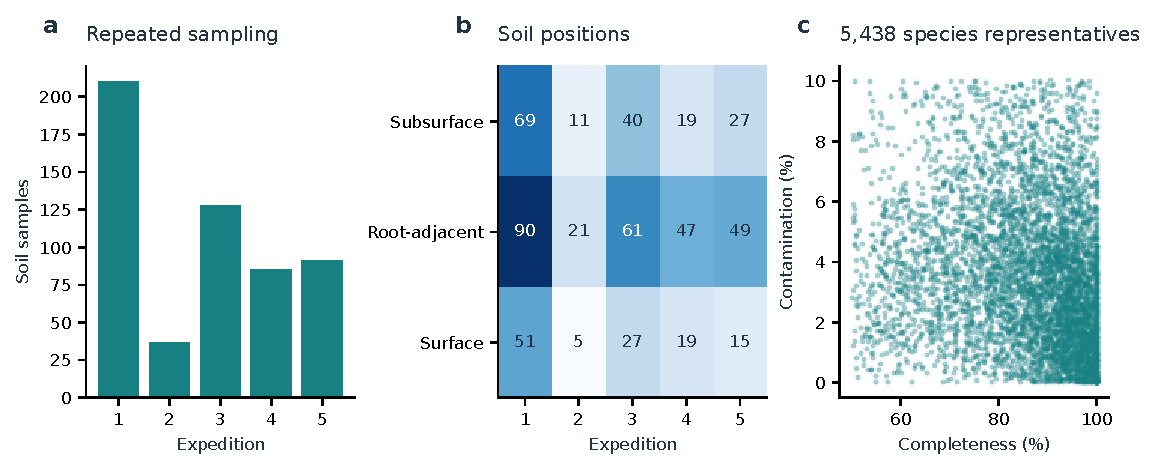
\includegraphics[width=\textwidth]{figures/fig_study_current.pdf}
\caption{\textbf{Sampling and genome quality.} \textbf{a}, Counts of the 551 soil samples
across five expeditions. \textbf{b}, Sample counts by soil position and expedition.
\textbf{c}, CheckM2 completeness and contamination for the 5{,}438 species representatives.
Sampling covers 59 core sites and two auxiliary locations; expedition and position counts describe samples, while the quality
panel describes dereplicated genomes.}
\label{fig:design}
\end{figure}

\begin{figure}[p]\centering
\includegraphics[width=0.90\textwidth]{figures/fig_dark_current.pdf}
\caption{\textbf{Sequence conservation in recurrent families and sharing with cultured bacteria.}
\textbf{a}, Empirical cumulative distributions of family median dN/dS for 97{,}200 dark and
95{,}647 annotated families. The display extends to dN/dS = 2; cumulative fractions use all families.
\textbf{b}, Annotated- and shifted-frame calibration distributions from a 10{,}000-family input,
with 9{,}182 and 9{,}148 evaluable outputs; the display extends to dN/dS = 3.
\textbf{c}, Difference between dark and annotated family medians in left-closed divergence strata (final bin includes 2), with 95\% intervals from 1,000 family bootstrap replicates. Labels give dark/control counts. Intervals use independent family resampling.
\textbf{d}, Percentage of annotated and dark MAG protein calls with reciprocal protein hits
in the paired culture-derived assembly, for 22 species groups after exclusion of a confirmed
\emph{E. coli} contaminant. Each line joins the two fractions for one MAG. \textbf{e}, DNA support by protein-hit status, with counts above bars. Eligible coding intervals are at least 90 nt; support requires a base-level alignment at 95\% identity and 90\% query coverage. \textbf{f}, Recovery of protein-shared calls by genome pair; the dotted line marks a post hoc 90\% diagnostic threshold.}
\label{fig:dark}
\end{figure}

\begin{figure}[p]\centering
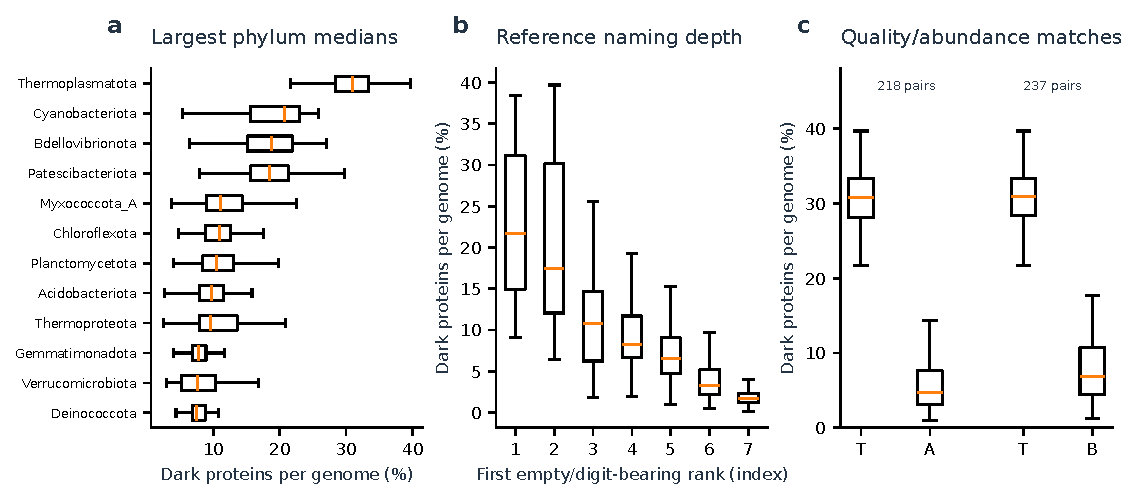
\includegraphics[width=\textwidth]{figures/fig_lineage_current.pdf}
\caption{\textbf{Thermoplasmatota carry high fractions of unknown proteins.} \textbf{a}, The twelve
highest median dark fractions among phyla with at least 20 representatives. \textbf{b}, Dark
fraction by the first empty or digit-bearing label: 1, phylum; 2, class; 3, order; 4, family;
5, genus; 6, species; 7, no flagged rank. \textbf{c}, Thermoplasmatota (T) and matched other
archaea (A) or bacteria (B), matched on completeness, contamination, corrected genome size,
N50, abundance and prevalence. The archaeal and bacterial matching sets have separate target
subsets (218 and 237 pairs). Boxes show the median and interquartile range; whiskers extend to 1.5 interquartile
ranges, and points beyond the whiskers are omitted.}
\label{fig:lineage}
\end{figure}

\begin{figure}[p]\centering
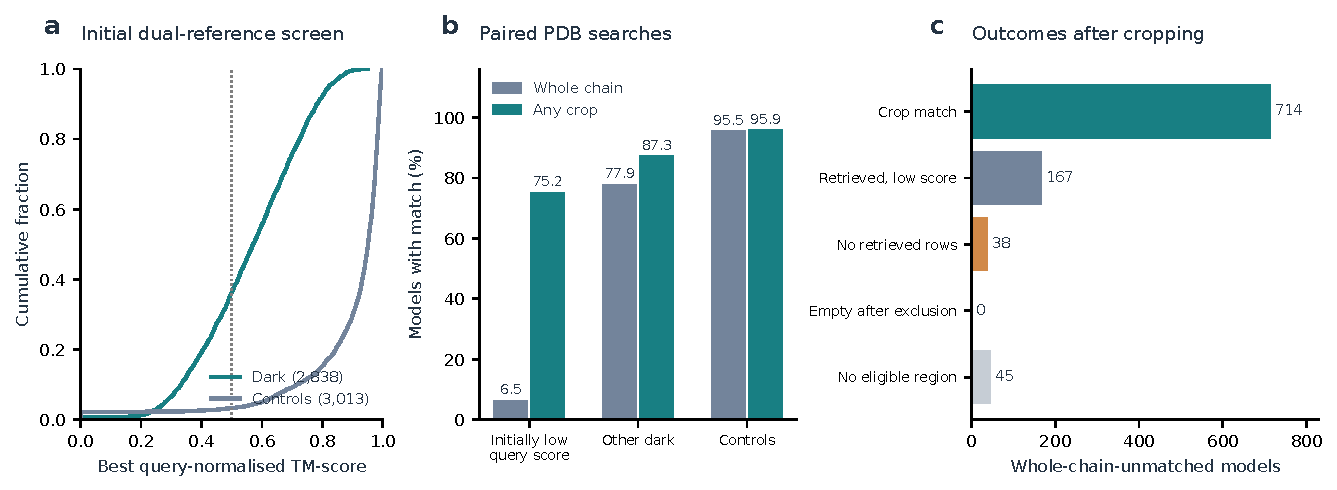
\includegraphics[width=\textwidth]{figures/fig_structure_current.pdf}
\caption{\textbf{Known structural features occur within sequence-dark proteins.}
\textbf{a}, Best query-normalised TM-score across the initial PDB and AlphaFold references
for 2{,}838 qualified dark models and 3{,}013 controls. The dashed line marks 0.5; zero retrievals
are retained at zero. \textbf{b}, Whole-chain and any-crop match fractions in the paired CPU
PDB search, with source entries excluded for controls. The initial low-query-score dark group
contains 1{,}031 models and the other dark group 1{,}807; all models remain in the denominator,
including those with no eligible region. The initial screen used both PDB and AlphaFold
references; the paired experiment used a newer PDB snapshot and greater retrieval depth.
These changes allow whole-chain classifications to differ between panels a and b. \textbf{c}, Paired outcomes among the 964 same-run
whole-chain-unmatched models in the initial low-query-score dark group. Crops recover matches
for 714; the remaining categories separate search and region-selection outcomes.}
\label{fig:structural}
\end{figure}

\begin{figure}[p]\centering
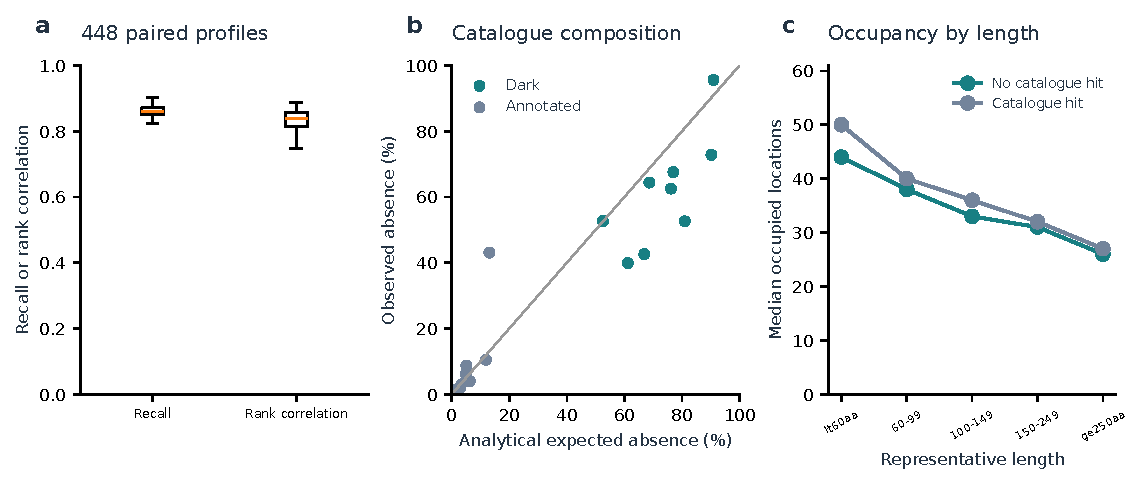
\includegraphics[width=\textwidth]{figures/fig_reference_current.pdf}
\caption{\textbf{Soil references recover widely distributed dark families.} \textbf{a}, Presence-recall of genome-encoded orthologues and rank correlation on shared orthologues across 448 paired profiles. PICRUSt2 emits its full orthologue set in 419 samples at the greater-than-zero threshold; recall therefore largely reflects reference overlap. Boxes show medians and interquartile ranges, with 1.5-interquartile-range whiskers and outliers omitted. \textbf{b}, Observed absence versus the analytical E-value-corrected MGnify90 rarefaction expectation at the indexed catalogue sizes, except the retained SPIRE expectation uses a 271.0-million-sequence anchor for its 269.5-million-sequence index. The diagonal indicates agreement with the size-only expectation. Each point is a catalogue, coloured by query group; points below the diagonal have lower observed absence. Atacama has 4.67 percentage points more dark-family absence and 29.97 points more annotated-family absence than the size-only expectation, demonstrating a large reference-composition residual. The combined desert and SPIRE annotated residuals are +0.93 and +1.23 points in expected-minus-observed absence. \textbf{c}, Median occupied locations out of 61, stratified by representative length and absence from every searched catalogue. }
\label{fig:reference}
\end{figure}




\begin{figure}[p]\centering
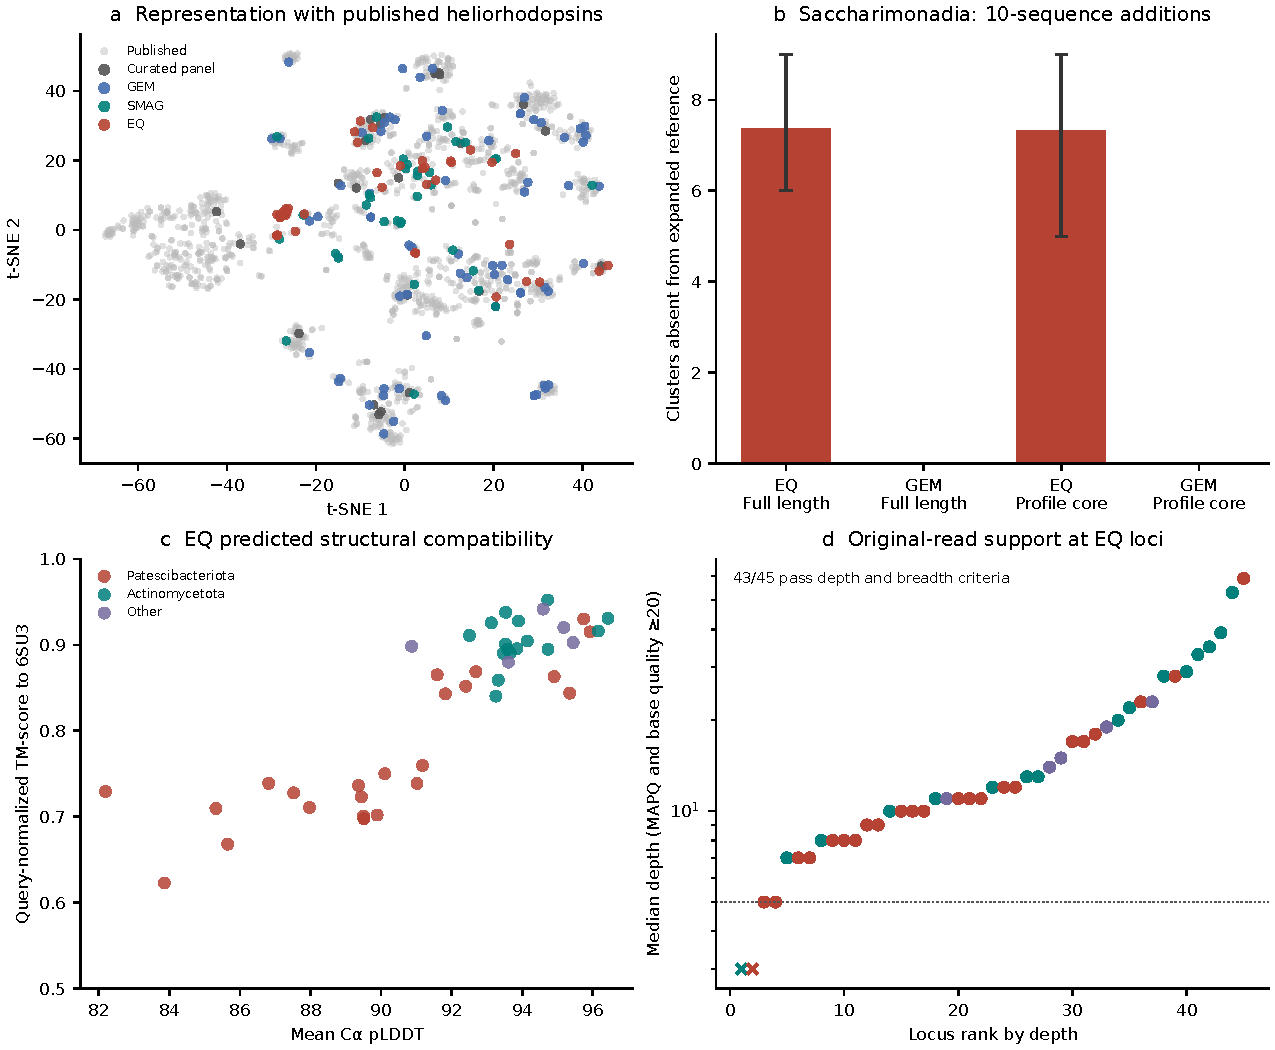
\includegraphics[width=\textwidth]{figures/fig_helio_expanded.pdf}
\caption{\textbf{Desert heliorhodopsins extend sequence diversity around a known fold.} \textbf{a}, ProstT5 t-SNE projection of 1{,}726 unique sequences from the Rub' al-Khali, sampled SMAG/GEM, curated and expanded published panels. The projection displays relationships among the encoded sequences. \textbf{b}, Mean numbers of 50\%-identity clusters absent from the expanded reference after adding ten Saccharimonadia sequences; error bars show the 2.5th--97.5th percentiles of 1{,}000 draws from the fixed source panels. Full-length and profile-core partitions use identical input records. GEM overlaps the published panel, including eight of its 73 source records exactly; zero added clusters indicates coverage by this reference panel. \textbf{c}, Mean C$\alpha$ pLDDT and full-query-normalised TM-score to 6SU3 for 45 Rub' al-Khali models. Terminal extensions contribute to the query-length denominator. These predictions are sequence-derived evidence of fold compatibility. \textbf{d}, Median quality-filtered depth at the 45 Rub' al-Khali loci in original assembly mappings. Crosses mark the two loci failing the depth/breadth rule; the dotted line is depth five. Colours in c and d indicate host phylum.}
\label{fig:helio}
\end{figure}

\bibliographystyle{unsrtnat}
\bibliography{references}

\end{document}
